\documentclass[twoside]{book}

% Packages required by doxygen
\usepackage{fixltx2e}
\usepackage{calc}
\usepackage{doxygen}
\usepackage[export]{adjustbox} % also loads graphicx
\usepackage{graphicx}
\usepackage[utf8]{inputenc}
\usepackage{makeidx}
\usepackage{multicol}
\usepackage{multirow}
\PassOptionsToPackage{warn}{textcomp}
\usepackage{textcomp}
\usepackage[nointegrals]{wasysym}
\usepackage[table]{xcolor}

% Font selection
\usepackage[T1]{fontenc}
\usepackage[scaled=.90]{helvet}
\usepackage{courier}
\usepackage{amssymb}
\usepackage{sectsty}
\renewcommand{\familydefault}{\sfdefault}
\allsectionsfont{%
  \fontseries{bc}\selectfont%
  \color{darkgray}%
}
\renewcommand{\DoxyLabelFont}{%
  \fontseries{bc}\selectfont%
  \color{darkgray}%
}
\newcommand{\+}{\discretionary{\mbox{\scriptsize$\hookleftarrow$}}{}{}}

% Page & text layout
\usepackage{geometry}
\geometry{%
  a4paper,%
  top=2.5cm,%
  bottom=2.5cm,%
  left=2.5cm,%
  right=2.5cm%
}
\tolerance=750
\hfuzz=15pt
\hbadness=750
\setlength{\emergencystretch}{15pt}
\setlength{\parindent}{0cm}
\setlength{\parskip}{3ex plus 2ex minus 2ex}
\makeatletter
\renewcommand{\paragraph}{%
  \@startsection{paragraph}{4}{0ex}{-1.0ex}{1.0ex}{%
    \normalfont\normalsize\bfseries\SS@parafont%
  }%
}
\renewcommand{\subparagraph}{%
  \@startsection{subparagraph}{5}{0ex}{-1.0ex}{1.0ex}{%
    \normalfont\normalsize\bfseries\SS@subparafont%
  }%
}
\makeatother

% Headers & footers
\usepackage{fancyhdr}
\pagestyle{fancyplain}
\fancyhead[LE]{\fancyplain{}{\bfseries\thepage}}
\fancyhead[CE]{\fancyplain{}{}}
\fancyhead[RE]{\fancyplain{}{\bfseries\leftmark}}
\fancyhead[LO]{\fancyplain{}{\bfseries\rightmark}}
\fancyhead[CO]{\fancyplain{}{}}
\fancyhead[RO]{\fancyplain{}{\bfseries\thepage}}
\fancyfoot[LE]{\fancyplain{}{}}
\fancyfoot[CE]{\fancyplain{}{}}
\fancyfoot[RE]{\fancyplain{}{\bfseries\scriptsize Generated by Doxygen }}
\fancyfoot[LO]{\fancyplain{}{\bfseries\scriptsize Generated by Doxygen }}
\fancyfoot[CO]{\fancyplain{}{}}
\fancyfoot[RO]{\fancyplain{}{}}
\renewcommand{\footrulewidth}{0.4pt}
\renewcommand{\chaptermark}[1]{%
  \markboth{#1}{}%
}
\renewcommand{\sectionmark}[1]{%
  \markright{\thesection\ #1}%
}

% Indices & bibliography
\usepackage{natbib}
\usepackage[titles]{tocloft}
\setcounter{tocdepth}{3}
\setcounter{secnumdepth}{5}
\makeindex

% Hyperlinks (required, but should be loaded last)
\usepackage{ifpdf}
\ifpdf
  \usepackage[pdftex,pagebackref=true]{hyperref}
\else
  \usepackage[ps2pdf,pagebackref=true]{hyperref}
\fi
\hypersetup{%
  colorlinks=true,%
  linkcolor=blue,%
  citecolor=blue,%
  unicode%
}

% Custom commands
\newcommand{\clearemptydoublepage}{%
  \newpage{\pagestyle{empty}\cleardoublepage}%
}

\usepackage{caption}
\captionsetup{labelsep=space,justification=centering,font={bf},singlelinecheck=off,skip=4pt,position=top}

%===== C O N T E N T S =====

\begin{document}

% Titlepage & ToC
\hypersetup{pageanchor=false,
             bookmarksnumbered=true,
             pdfencoding=unicode
            }
\pagenumbering{roman}
\begin{titlepage}
\vspace*{7cm}
\begin{center}%
{\Large My Project }\\
\vspace*{1cm}
{\large Generated by Doxygen 1.8.11}\\
\end{center}
\end{titlepage}
\clearemptydoublepage
\tableofcontents
\clearemptydoublepage
\pagenumbering{arabic}
\hypersetup{pageanchor=true}

%--- Begin generated contents ---
\chapter{Hierarchical Index}
\section{Class Hierarchy}
This inheritance list is sorted roughly, but not completely, alphabetically\+:\begin{DoxyCompactList}
\item \contentsline{section}{Date}{\pageref{class_date}}{}
\begin{DoxyCompactList}
\item \contentsline{section}{Date\+Offset}{\pageref{class_date_offset}}{}
\end{DoxyCompactList}
\item \contentsline{section}{Item}{\pageref{class_item}}{}
\item \contentsline{section}{Member}{\pageref{class_member}}{}
\item \contentsline{section}{Item\+:\+:Purchase}{\pageref{class_item_1_1_purchase}}{}
\item Q\+Dialog\begin{DoxyCompactList}
\item \contentsline{section}{New\+Item}{\pageref{class_new_item}}{}
\item \contentsline{section}{New\+Member}{\pageref{class_new_member}}{}
\end{DoxyCompactList}
\item Q\+Main\+Window\begin{DoxyCompactList}
\item \contentsline{section}{Main\+Window}{\pageref{class_main_window}}{}
\end{DoxyCompactList}
\end{DoxyCompactList}

\chapter{Class Index}
\section{Class List}
Here are the classes, structs, unions and interfaces with brief descriptions\+:\begin{DoxyCompactList}
\item\contentsline{section}{\hyperlink{class_date}{Date} }{\pageref{class_date}}{}
\item\contentsline{section}{\hyperlink{class_date_offset}{Date\+Offset} }{\pageref{class_date_offset}}{}
\item\contentsline{section}{\hyperlink{class_item}{Item} }{\pageref{class_item}}{}
\item\contentsline{section}{\hyperlink{class_main_window}{Main\+Window} }{\pageref{class_main_window}}{}
\item\contentsline{section}{\hyperlink{class_member}{Member} }{\pageref{class_member}}{}
\item\contentsline{section}{\hyperlink{class_new_item}{New\+Item} }{\pageref{class_new_item}}{}
\item\contentsline{section}{\hyperlink{class_new_member}{New\+Member} }{\pageref{class_new_member}}{}
\item\contentsline{section}{\hyperlink{class_item_1_1_purchase}{Item\+::\+Purchase} }{\pageref{class_item_1_1_purchase}}{}
\end{DoxyCompactList}

\chapter{Class Documentation}
\hypertarget{class_binomial}{}\section{Binomial$<$ First\+\_\+\+Type, Secnd\+\_\+\+Type $>$ Class Template Reference}
\label{class_binomial}\index{Binomial$<$ First\+\_\+\+Type, Secnd\+\_\+\+Type $>$@{Binomial$<$ First\+\_\+\+Type, Secnd\+\_\+\+Type $>$}}


The \hyperlink{class_binomial}{Binomial} class Puts two pointers together to let the user access both.  




{\ttfamily \#include $<$Binomial.\+h$>$}

\subsection*{Public Member Functions}
\begin{DoxyCompactItemize}
\item 
\hyperlink{class_binomial_af09d420e38603496bf3bef29332e5828}{Binomial} ()
\begin{DoxyCompactList}\small\item\em This is a default constructor. \end{DoxyCompactList}\item 
\hyperlink{class_binomial_a124e073e89f235b8b62ffbe0c0b65472}{Binomial} (First\+\_\+\+Type $\ast$first\+Ptr, Secnd\+\_\+\+Type $\ast$secnd\+Ptr)
\begin{DoxyCompactList}\small\item\em This is a nondefault constructor. \end{DoxyCompactList}\item 
\hyperlink{class_binomial_abe3263cfb456f2b3b2e0e3486f7cd45c}{$\sim$\+Binomial} ()
\begin{DoxyCompactList}\small\item\em This is a default deconstructor. \end{DoxyCompactList}\item 
First\+\_\+\+Type $\ast$\& \hyperlink{class_binomial_a21c033051a572ed5339f37f085c7ffc9}{First\+Ptr} ()
\begin{DoxyCompactList}\small\item\em First\+Ptr return. \end{DoxyCompactList}\item 
Secnd\+\_\+\+Type $\ast$\& \hyperlink{class_binomial_a5cbb90adb595570afa8a4ffe5fadad3a}{Secnd\+Ptr} ()
\begin{DoxyCompactList}\small\item\em Secnd\+Ptr return. \end{DoxyCompactList}\item 
const First\+\_\+\+Type $\ast$\& \hyperlink{class_binomial_a0efc152a49648b63b5b52a4170535336}{First\+Ptr} () const 
\begin{DoxyCompactList}\small\item\em const First\+Ptr return \end{DoxyCompactList}\item 
const Secnd\+\_\+\+Type $\ast$\& \hyperlink{class_binomial_a4c52d21a8a0395fb486907b2ab35999b}{Secnd\+Ptr} () const 
\begin{DoxyCompactList}\small\item\em const Secnd\+Ptr return \end{DoxyCompactList}\end{DoxyCompactItemize}


\subsection{Detailed Description}
\subsubsection*{template$<$typename First\+\_\+\+Type, typename Secnd\+\_\+\+Type$>$\\*
class Binomial$<$ First\+\_\+\+Type, Secnd\+\_\+\+Type $>$}

The \hyperlink{class_binomial}{Binomial} class Puts two pointers together to let the user access both. 

T\+E\+M\+P\+L\+A\+TE C\+L\+A\+SS\+: Binomail 

 The \hyperlink{class_binomial}{Binomial} class puts two pointers together and allows the user to access the data that is stored in them. 

\subsection{Constructor \& Destructor Documentation}
\index{Binomial@{Binomial}!Binomial@{Binomial}}
\index{Binomial@{Binomial}!Binomial@{Binomial}}
\subsubsection[{\texorpdfstring{Binomial()}{Binomial()}}]{\setlength{\rightskip}{0pt plus 5cm}template$<$typename First\+\_\+\+Type, typename Secnd\+\_\+\+Type$>$ {\bf Binomial}$<$ First\+\_\+\+Type, Secnd\+\_\+\+Type $>$\+::{\bf Binomial} (
\begin{DoxyParamCaption}
{}
\end{DoxyParamCaption}
)\hspace{0.3cm}{\ttfamily [inline]}}\hypertarget{class_binomial_af09d420e38603496bf3bef29332e5828}{}\label{class_binomial_af09d420e38603496bf3bef29332e5828}


This is a default constructor. 

This constructor does nothing \index{Binomial@{Binomial}!Binomial@{Binomial}}
\index{Binomial@{Binomial}!Binomial@{Binomial}}
\subsubsection[{\texorpdfstring{Binomial(\+First\+\_\+\+Type $\ast$first\+Ptr, Secnd\+\_\+\+Type $\ast$secnd\+Ptr)}{Binomial(First_Type *firstPtr, Secnd_Type *secndPtr)}}]{\setlength{\rightskip}{0pt plus 5cm}template$<$typename First\+\_\+\+Type, typename Secnd\+\_\+\+Type$>$ {\bf Binomial}$<$ First\+\_\+\+Type, Secnd\+\_\+\+Type $>$\+::{\bf Binomial} (
\begin{DoxyParamCaption}
\item[{First\+\_\+\+Type $\ast$}]{first\+Ptr, }
\item[{Secnd\+\_\+\+Type $\ast$}]{secnd\+Ptr}
\end{DoxyParamCaption}
)\hspace{0.3cm}{\ttfamily [inline]}}\hypertarget{class_binomial_a124e073e89f235b8b62ffbe0c0b65472}{}\label{class_binomial_a124e073e89f235b8b62ffbe0c0b65472}


This is a nondefault constructor. 

This constructor sets the arguments equal to the private pointer variables in this class \index{Binomial@{Binomial}!````~Binomial@{$\sim$\+Binomial}}
\index{````~Binomial@{$\sim$\+Binomial}!Binomial@{Binomial}}
\subsubsection[{\texorpdfstring{$\sim$\+Binomial()}{~Binomial()}}]{\setlength{\rightskip}{0pt plus 5cm}template$<$typename First\+\_\+\+Type, typename Secnd\+\_\+\+Type$>$ {\bf Binomial}$<$ First\+\_\+\+Type, Secnd\+\_\+\+Type $>$\+::$\sim${\bf Binomial} (
\begin{DoxyParamCaption}
{}
\end{DoxyParamCaption}
)\hspace{0.3cm}{\ttfamily [inline]}}\hypertarget{class_binomial_abe3263cfb456f2b3b2e0e3486f7cd45c}{}\label{class_binomial_abe3263cfb456f2b3b2e0e3486f7cd45c}


This is a default deconstructor. 

This deconstructor does nothing 

\subsection{Member Function Documentation}
\index{Binomial@{Binomial}!First\+Ptr@{First\+Ptr}}
\index{First\+Ptr@{First\+Ptr}!Binomial@{Binomial}}
\subsubsection[{\texorpdfstring{First\+Ptr()}{FirstPtr()}}]{\setlength{\rightskip}{0pt plus 5cm}template$<$typename First\+\_\+\+Type, typename Secnd\+\_\+\+Type$>$ First\+\_\+\+Type$\ast$\& {\bf Binomial}$<$ First\+\_\+\+Type, Secnd\+\_\+\+Type $>$\+::First\+Ptr (
\begin{DoxyParamCaption}
{}
\end{DoxyParamCaption}
)\hspace{0.3cm}{\ttfamily [inline]}}\hypertarget{class_binomial_a21c033051a572ed5339f37f085c7ffc9}{}\label{class_binomial_a21c033051a572ed5339f37f085c7ffc9}


First\+Ptr return. 

This returns what the First\+Ptr is pointing to \index{Binomial@{Binomial}!First\+Ptr@{First\+Ptr}}
\index{First\+Ptr@{First\+Ptr}!Binomial@{Binomial}}
\subsubsection[{\texorpdfstring{First\+Ptr() const }{FirstPtr() const }}]{\setlength{\rightskip}{0pt plus 5cm}template$<$typename First\+\_\+\+Type, typename Secnd\+\_\+\+Type$>$ const First\+\_\+\+Type$\ast$\& {\bf Binomial}$<$ First\+\_\+\+Type, Secnd\+\_\+\+Type $>$\+::First\+Ptr (
\begin{DoxyParamCaption}
{}
\end{DoxyParamCaption}
) const\hspace{0.3cm}{\ttfamily [inline]}}\hypertarget{class_binomial_a0efc152a49648b63b5b52a4170535336}{}\label{class_binomial_a0efc152a49648b63b5b52a4170535336}


const First\+Ptr return 

This returns what the First\+Ptr is pointing to, this will be called upon if the template is defined as a constant \index{Binomial@{Binomial}!Secnd\+Ptr@{Secnd\+Ptr}}
\index{Secnd\+Ptr@{Secnd\+Ptr}!Binomial@{Binomial}}
\subsubsection[{\texorpdfstring{Secnd\+Ptr()}{SecndPtr()}}]{\setlength{\rightskip}{0pt plus 5cm}template$<$typename First\+\_\+\+Type, typename Secnd\+\_\+\+Type$>$ Secnd\+\_\+\+Type$\ast$\& {\bf Binomial}$<$ First\+\_\+\+Type, Secnd\+\_\+\+Type $>$\+::Secnd\+Ptr (
\begin{DoxyParamCaption}
{}
\end{DoxyParamCaption}
)\hspace{0.3cm}{\ttfamily [inline]}}\hypertarget{class_binomial_a5cbb90adb595570afa8a4ffe5fadad3a}{}\label{class_binomial_a5cbb90adb595570afa8a4ffe5fadad3a}


Secnd\+Ptr return. 

This returns what the Secnd\+Ptr is pointing to \index{Binomial@{Binomial}!Secnd\+Ptr@{Secnd\+Ptr}}
\index{Secnd\+Ptr@{Secnd\+Ptr}!Binomial@{Binomial}}
\subsubsection[{\texorpdfstring{Secnd\+Ptr() const }{SecndPtr() const }}]{\setlength{\rightskip}{0pt plus 5cm}template$<$typename First\+\_\+\+Type, typename Secnd\+\_\+\+Type$>$ const Secnd\+\_\+\+Type$\ast$\& {\bf Binomial}$<$ First\+\_\+\+Type, Secnd\+\_\+\+Type $>$\+::Secnd\+Ptr (
\begin{DoxyParamCaption}
{}
\end{DoxyParamCaption}
) const\hspace{0.3cm}{\ttfamily [inline]}}\hypertarget{class_binomial_a4c52d21a8a0395fb486907b2ab35999b}{}\label{class_binomial_a4c52d21a8a0395fb486907b2ab35999b}


const Secnd\+Ptr return 

This returns what the Secnd\+Ptr is pointing to, this will be called upon if the template is defined as a constant 

The documentation for this class was generated from the following file\+:\begin{DoxyCompactItemize}
\item 
Binomial.\+h\end{DoxyCompactItemize}

\hypertarget{class_database}{}\section{Database Class Reference}
\label{class_database}\index{Database@{Database}}


The \hyperlink{class_database}{Database} class Is a wrapper for the sqlite database.  




{\ttfamily \#include $<$database.\+h$>$}

Inheritance diagram for Database\+:\begin{figure}[H]
\begin{center}
\leavevmode
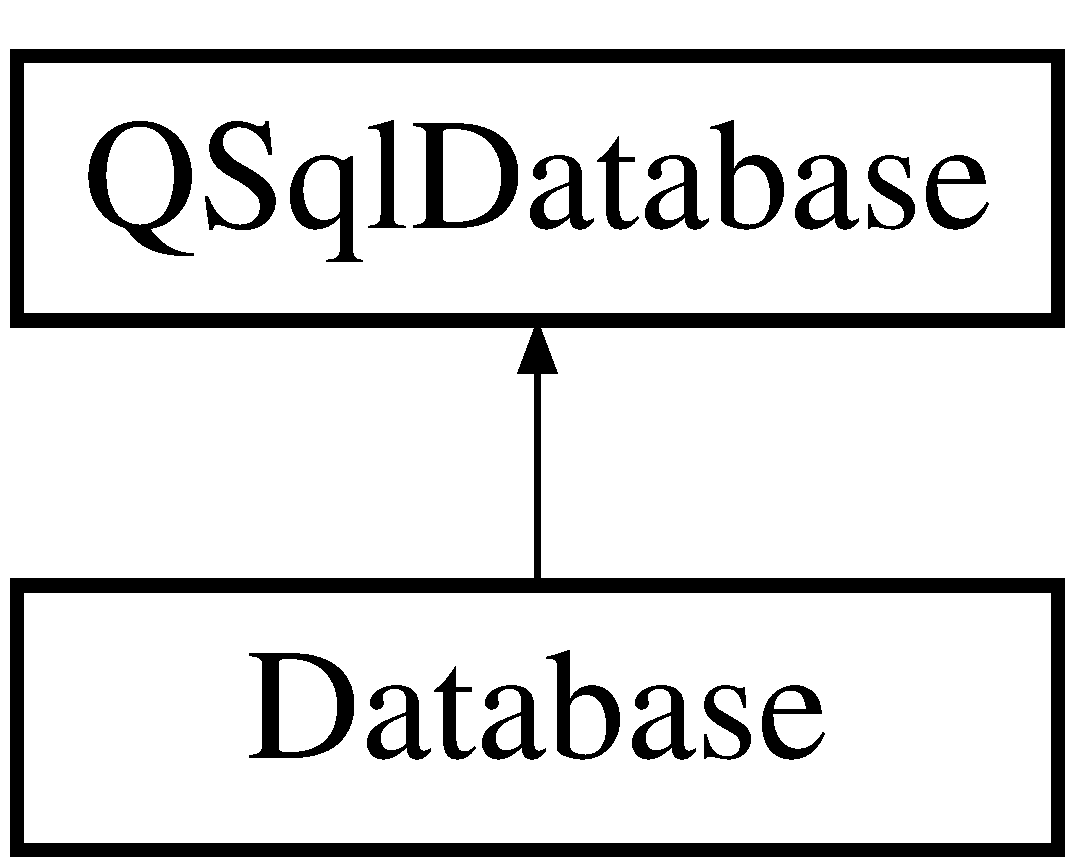
\includegraphics[height=2.000000cm]{class_database}
\end{center}
\end{figure}
\subsection*{Public Member Functions}
\begin{DoxyCompactItemize}
\item 
\hyperlink{class_database_a84d399a2ad58d69daab9b05330e1316d}{$\sim$\+Database} ()
\begin{DoxyCompactList}\small\item\em This is a default deconstructor. \end{DoxyCompactList}\item 
void \hyperlink{class_database_a758e61f68f8c15b1cbce3a33a7cf47d6}{Add\+Item} (\hyperlink{class_item}{Item} item)
\begin{DoxyCompactList}\small\item\em Adds a new item to the database. \end{DoxyCompactList}\item 
void \hyperlink{class_database_a30727815c52554ab2c16241a800cad4a}{Update\+Item} (\hyperlink{class_item}{Item} item)
\begin{DoxyCompactList}\small\item\em Update an item. \end{DoxyCompactList}\item 
bool \hyperlink{class_database_a78954f7fa149e4e8b3e67d16b25eaf95}{Delete\+Item} (int id)
\begin{DoxyCompactList}\small\item\em Deletes an item. \end{DoxyCompactList}\item 
\hyperlink{class_item}{Item} \hyperlink{class_database_a6a08b00282577ba5872e5d204a3a8a1f}{Get\+Item\+By\+ID} (int id)
\begin{DoxyCompactList}\small\item\em Gets an item by checking the input ID. \end{DoxyCompactList}\item 
Q\+Sql\+Table\+Model $\ast$ \hyperlink{class_database_af31b0f441345116776e4f79c3944b3c9}{Get\+All\+Items} ()
\begin{DoxyCompactList}\small\item\em Gets all items from the database. \end{DoxyCompactList}\item 
void \hyperlink{class_database_a9989a7c15d345e2158795ae5e07fe162}{Add\+User} (\hyperlink{class_member}{Member} member)
\begin{DoxyCompactList}\small\item\em Adds a user to the database. \end{DoxyCompactList}\item 
Q\+Sql\+Table\+Model $\ast$ \hyperlink{class_database_a814cf5256dbd1660e3db8beb3a49ebf1}{Get\+All\+Members} ()
\begin{DoxyCompactList}\small\item\em Gets all of the members from the database. \end{DoxyCompactList}\item 
Q\+Sql\+Table\+Model $\ast$ \hyperlink{class_database_a68f574c4873b6687715bb0decc752ada}{Get\+Filtered\+Members} (Q\+String month)
\begin{DoxyCompactList}\small\item\em Gets all of the filtered members from the database. \end{DoxyCompactList}\item 
void \hyperlink{class_database_a908114ff4d6dc748ebdd2579ebd6c79c}{Add\+Purchase} (\hyperlink{class_purchase}{Purchase} purchase)
\begin{DoxyCompactList}\small\item\em Adds a purchase to the database. \end{DoxyCompactList}\item 
Q\+Sql\+Table\+Model $\ast$ \hyperlink{class_database_a9f87a20b8475c8f02845aaf5bf039cbe}{Get\+All\+Purchases} ()
\begin{DoxyCompactList}\small\item\em Gets all of the purchases from the database. \end{DoxyCompactList}\end{DoxyCompactItemize}
\subsection*{Static Public Member Functions}
\begin{DoxyCompactItemize}
\item 
static \hyperlink{class_database}{Database} $\ast$ \hyperlink{class_database_a263f3471515ca1bb7ea0a096f7502d49}{Get\+Instance} ()
\begin{DoxyCompactList}\small\item\em Gets a new database instance. \end{DoxyCompactList}\end{DoxyCompactItemize}


\subsection{Detailed Description}
The \hyperlink{class_database}{Database} class Is a wrapper for the sqlite database. 

C\+L\+A\+SS\+: \hyperlink{class_database}{Database} 

 This database class copies data over from sqlite and formats it to be used in cpp 

\subsection{Constructor \& Destructor Documentation}
\index{Database@{Database}!````~Database@{$\sim$\+Database}}
\index{````~Database@{$\sim$\+Database}!Database@{Database}}
\subsubsection[{\texorpdfstring{$\sim$\+Database()}{~Database()}}]{\setlength{\rightskip}{0pt plus 5cm}Database\+::$\sim$\+Database (
\begin{DoxyParamCaption}
{}
\end{DoxyParamCaption}
)}\hypertarget{class_database_a84d399a2ad58d69daab9b05330e1316d}{}\label{class_database_a84d399a2ad58d69daab9b05330e1316d}


This is a default deconstructor. 

This deconstructor deletes any dynamically allocated data for the class 

\subsection{Member Function Documentation}
\index{Database@{Database}!Add\+Item@{Add\+Item}}
\index{Add\+Item@{Add\+Item}!Database@{Database}}
\subsubsection[{\texorpdfstring{Add\+Item(\+Item item)}{AddItem(Item item)}}]{\setlength{\rightskip}{0pt plus 5cm}void Database\+::\+Add\+Item (
\begin{DoxyParamCaption}
\item[{{\bf Item}}]{item}
\end{DoxyParamCaption}
)}\hypertarget{class_database_a758e61f68f8c15b1cbce3a33a7cf47d6}{}\label{class_database_a758e61f68f8c15b1cbce3a33a7cf47d6}


Adds a new item to the database. 

This function inserts a new item in to the database by inserting a name, quantity, price, and onshelf \index{Database@{Database}!Add\+Purchase@{Add\+Purchase}}
\index{Add\+Purchase@{Add\+Purchase}!Database@{Database}}
\subsubsection[{\texorpdfstring{Add\+Purchase(\+Purchase purchase)}{AddPurchase(Purchase purchase)}}]{\setlength{\rightskip}{0pt plus 5cm}void Database\+::\+Add\+Purchase (
\begin{DoxyParamCaption}
\item[{{\bf Purchase}}]{purchase}
\end{DoxyParamCaption}
)}\hypertarget{class_database_a908114ff4d6dc748ebdd2579ebd6c79c}{}\label{class_database_a908114ff4d6dc748ebdd2579ebd6c79c}


Adds a purchase to the database. 

This function uses the argument purchase and adds it to the database \index{Database@{Database}!Add\+User@{Add\+User}}
\index{Add\+User@{Add\+User}!Database@{Database}}
\subsubsection[{\texorpdfstring{Add\+User(\+Member member)}{AddUser(Member member)}}]{\setlength{\rightskip}{0pt plus 5cm}void Database\+::\+Add\+User (
\begin{DoxyParamCaption}
\item[{{\bf Member}}]{member}
\end{DoxyParamCaption}
)}\hypertarget{class_database_a9989a7c15d345e2158795ae5e07fe162}{}\label{class_database_a9989a7c15d345e2158795ae5e07fe162}


Adds a user to the database. 

This function will use the member object passed in as an argument and then gets added to the database \index{Database@{Database}!Delete\+Item@{Delete\+Item}}
\index{Delete\+Item@{Delete\+Item}!Database@{Database}}
\subsubsection[{\texorpdfstring{Delete\+Item(int id)}{DeleteItem(int id)}}]{\setlength{\rightskip}{0pt plus 5cm}bool Database\+::\+Delete\+Item (
\begin{DoxyParamCaption}
\item[{int}]{id}
\end{DoxyParamCaption}
)}\hypertarget{class_database_a78954f7fa149e4e8b3e67d16b25eaf95}{}\label{class_database_a78954f7fa149e4e8b3e67d16b25eaf95}


Deletes an item. 

This function will check to see if there is data left to be exectued and return true , if not then it will return false \index{Database@{Database}!Get\+All\+Items@{Get\+All\+Items}}
\index{Get\+All\+Items@{Get\+All\+Items}!Database@{Database}}
\subsubsection[{\texorpdfstring{Get\+All\+Items()}{GetAllItems()}}]{\setlength{\rightskip}{0pt plus 5cm}Q\+Sql\+Table\+Model$\ast$ Database\+::\+Get\+All\+Items (
\begin{DoxyParamCaption}
{}
\end{DoxyParamCaption}
)}\hypertarget{class_database_af31b0f441345116776e4f79c3944b3c9}{}\label{class_database_af31b0f441345116776e4f79c3944b3c9}


Gets all items from the database. 

Creates a new Q\+Sql\+Table\+Model and selects all items to be put in to the new table \index{Database@{Database}!Get\+All\+Members@{Get\+All\+Members}}
\index{Get\+All\+Members@{Get\+All\+Members}!Database@{Database}}
\subsubsection[{\texorpdfstring{Get\+All\+Members()}{GetAllMembers()}}]{\setlength{\rightskip}{0pt plus 5cm}Q\+Sql\+Table\+Model$\ast$ Database\+::\+Get\+All\+Members (
\begin{DoxyParamCaption}
{}
\end{DoxyParamCaption}
)}\hypertarget{class_database_a814cf5256dbd1660e3db8beb3a49ebf1}{}\label{class_database_a814cf5256dbd1660e3db8beb3a49ebf1}


Gets all of the members from the database. 

This function creates a new Q\+Sql\+Table\+Model and selects all of the members to be put in to the new table \index{Database@{Database}!Get\+All\+Purchases@{Get\+All\+Purchases}}
\index{Get\+All\+Purchases@{Get\+All\+Purchases}!Database@{Database}}
\subsubsection[{\texorpdfstring{Get\+All\+Purchases()}{GetAllPurchases()}}]{\setlength{\rightskip}{0pt plus 5cm}Q\+Sql\+Table\+Model$\ast$ Database\+::\+Get\+All\+Purchases (
\begin{DoxyParamCaption}
{}
\end{DoxyParamCaption}
)}\hypertarget{class_database_a9f87a20b8475c8f02845aaf5bf039cbe}{}\label{class_database_a9f87a20b8475c8f02845aaf5bf039cbe}


Gets all of the purchases from the database. 

This function creates a new Q\+Sql\+Table\+Model and selects all of the filtered members to be put in to the new table \index{Database@{Database}!Get\+Filtered\+Members@{Get\+Filtered\+Members}}
\index{Get\+Filtered\+Members@{Get\+Filtered\+Members}!Database@{Database}}
\subsubsection[{\texorpdfstring{Get\+Filtered\+Members(\+Q\+String month)}{GetFilteredMembers(QString month)}}]{\setlength{\rightskip}{0pt plus 5cm}Q\+Sql\+Table\+Model$\ast$ Database\+::\+Get\+Filtered\+Members (
\begin{DoxyParamCaption}
\item[{Q\+String}]{month}
\end{DoxyParamCaption}
)}\hypertarget{class_database_a68f574c4873b6687715bb0decc752ada}{}\label{class_database_a68f574c4873b6687715bb0decc752ada}


Gets all of the filtered members from the database. 

This function creates a new Q\+Sql\+Table\+Model and selects all of the filtered members to be put in to the new table \index{Database@{Database}!Get\+Instance@{Get\+Instance}}
\index{Get\+Instance@{Get\+Instance}!Database@{Database}}
\subsubsection[{\texorpdfstring{Get\+Instance()}{GetInstance()}}]{\setlength{\rightskip}{0pt plus 5cm}static {\bf Database}$\ast$ Database\+::\+Get\+Instance (
\begin{DoxyParamCaption}
{}
\end{DoxyParamCaption}
)\hspace{0.3cm}{\ttfamily [static]}}\hypertarget{class_database_a263f3471515ca1bb7ea0a096f7502d49}{}\label{class_database_a263f3471515ca1bb7ea0a096f7502d49}


Gets a new database instance. 

This constructor return a new instance of the database \index{Database@{Database}!Get\+Item\+By\+ID@{Get\+Item\+By\+ID}}
\index{Get\+Item\+By\+ID@{Get\+Item\+By\+ID}!Database@{Database}}
\subsubsection[{\texorpdfstring{Get\+Item\+By\+I\+D(int id)}{GetItemByID(int id)}}]{\setlength{\rightskip}{0pt plus 5cm}{\bf Item} Database\+::\+Get\+Item\+By\+ID (
\begin{DoxyParamCaption}
\item[{int}]{id}
\end{DoxyParamCaption}
)}\hypertarget{class_database_a6a08b00282577ba5872e5d204a3a8a1f}{}\label{class_database_a6a08b00282577ba5872e5d204a3a8a1f}


Gets an item by checking the input ID. 

This function checks the item ID until it finds a match and then returns the item \index{Database@{Database}!Update\+Item@{Update\+Item}}
\index{Update\+Item@{Update\+Item}!Database@{Database}}
\subsubsection[{\texorpdfstring{Update\+Item(\+Item item)}{UpdateItem(Item item)}}]{\setlength{\rightskip}{0pt plus 5cm}void Database\+::\+Update\+Item (
\begin{DoxyParamCaption}
\item[{{\bf Item}}]{item}
\end{DoxyParamCaption}
)}\hypertarget{class_database_a30727815c52554ab2c16241a800cad4a}{}\label{class_database_a30727815c52554ab2c16241a800cad4a}


Update an item. 

This function uses values from the item in the argument and transfers the data in to the database 

The documentation for this class was generated from the following file\+:\begin{DoxyCompactItemize}
\item 
database.\+h\end{DoxyCompactItemize}

\hypertarget{class_date}{}\section{Date Class Reference}
\label{class_date}\index{Date@{Date}}


Has a format for the date.  




{\ttfamily \#include $<$Date.\+h$>$}

Inheritance diagram for Date\+:\begin{figure}[H]
\begin{center}
\leavevmode
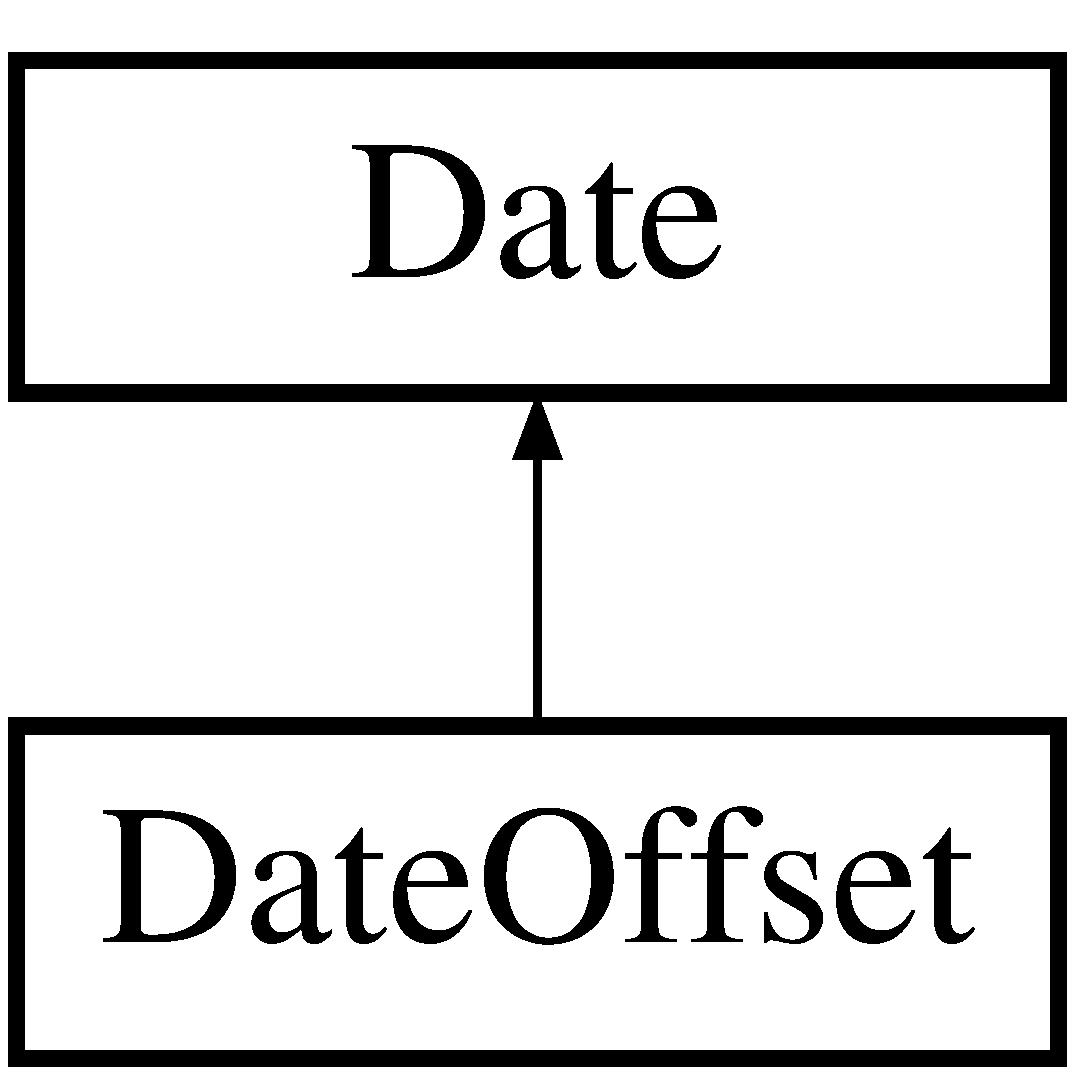
\includegraphics[height=2.000000cm]{class_date}
\end{center}
\end{figure}
\subsection*{Public Member Functions}
\begin{DoxyCompactItemize}
\item 
\hyperlink{class_date_a4e59ed4ba66eec61c27460c5d09fa1bd}{Date} ()
\begin{DoxyCompactList}\small\item\em This is the default date constructor. \end{DoxyCompactList}\item 
\hyperlink{class_date_afa65693475fb86a2de04c8578b232201}{Date} (const \hyperlink{class_date}{Date} \&)
\begin{DoxyCompactList}\small\item\em This is a copy class date constructor. \end{DoxyCompactList}\item 
\hyperlink{class_date_a5874432b5f7339205866055201e885d7}{Date} (int year, int month, int day)
\begin{DoxyCompactList}\small\item\em This is a non default date constructor. \end{DoxyCompactList}\item 
\hyperlink{class_date_ade4b469433b7966cc034cbcc6799233b}{$\sim$\+Date} ()
\begin{DoxyCompactList}\small\item\em This is the default date deconstructor. \end{DoxyCompactList}\item 
int \hyperlink{class_date_a3b9f9ebc5d79571606b30363b6121386}{Year} () const 
\begin{DoxyCompactList}\small\item\em Year return. \end{DoxyCompactList}\item 
int \hyperlink{class_date_a173d22f7c4671d3ad54b76994913967e}{Month} () const 
\begin{DoxyCompactList}\small\item\em Month return. \end{DoxyCompactList}\item 
int \hyperlink{class_date_a471379b5d940e5f8231d083e308110b9}{Day} () const 
\begin{DoxyCompactList}\small\item\em Day return. \end{DoxyCompactList}\item 
Q\+String \hyperlink{class_date_a4ba2694d9bbd84819322e8ed2fb112a5}{To\+String} (Q\+String format) const 
\begin{DoxyCompactList}\small\item\em Returns a qstring thats properly formatted from the individual int values. \end{DoxyCompactList}\item 
bool \hyperlink{class_date_ad54d8e4b8f2ad6df8eda3b8615c3c0b2}{operator==} (const \hyperlink{class_date}{Date} \&) const 
\begin{DoxyCompactList}\small\item\em Overloaded operator ==. \end{DoxyCompactList}\item 
bool \hyperlink{class_date_adc801e7b23c84cd65dd70a9ac76344e3}{operator!=} (const \hyperlink{class_date}{Date} \&) const 
\begin{DoxyCompactList}\small\item\em Overloaded operator !=. \end{DoxyCompactList}\item 
bool \hyperlink{class_date_a691bafd5bba9540f3c540f7327a758c2}{operator$<$} (const \hyperlink{class_date}{Date} \&) const 
\begin{DoxyCompactList}\small\item\em Overloaded operator $<$. \end{DoxyCompactList}\item 
bool \hyperlink{class_date_a0bd06d545842c948cdca8ccc60d7d68d}{operator$>$} (const \hyperlink{class_date}{Date} \&) const 
\begin{DoxyCompactList}\small\item\em Overloaded operator $>$ \end{DoxyCompactList}\item 
bool \hyperlink{class_date_a6632fd56fe1c549ef0a257c85fd8eb3e}{operator$<$=} (const \hyperlink{class_date}{Date} \&) const 
\begin{DoxyCompactList}\small\item\em Overloaded operator $<$=. \end{DoxyCompactList}\item 
bool \hyperlink{class_date_ae4802fa52cf81f1a259b4a3b88bffc0d}{operator$>$=} (const \hyperlink{class_date}{Date} \&) const 
\begin{DoxyCompactList}\small\item\em Overloaded operator $>$=. \end{DoxyCompactList}\item 
\hyperlink{class_date}{Date} \& \hyperlink{class_date_ab07c405865e57d005249355e7912a09c}{operator+=} (const \hyperlink{class_date_offset}{Date\+Offset} \&)
\begin{DoxyCompactList}\small\item\em Overloaded operator +=. \end{DoxyCompactList}\item 
\hyperlink{class_date}{Date} \& \hyperlink{class_date_aadaf96a289eaacffde684367ee1a8770}{operator-\/=} (const \hyperlink{class_date_offset}{Date\+Offset} \&)
\begin{DoxyCompactList}\small\item\em Overloaded operator -\/=. \end{DoxyCompactList}\item 
const \hyperlink{class_date}{Date} \hyperlink{class_date_a76fb6c5f25f2edb5408966f769a378e1}{operator+} (const \hyperlink{class_date_offset}{Date\+Offset} \&) const 
\begin{DoxyCompactList}\small\item\em Overloaded operator +. \end{DoxyCompactList}\item 
const \hyperlink{class_date}{Date} \hyperlink{class_date_ac979d70d595be12cc3bde83149cbe33e}{operator-\/} (const \hyperlink{class_date_offset}{Date\+Offset} \&) const 
\begin{DoxyCompactList}\small\item\em Overloaded operator -\/. \end{DoxyCompactList}\item 
const \hyperlink{class_date_offset}{Date\+Offset} \hyperlink{class_date_a4030ca7cef26e292fc070817e9ee3392}{operator+} (const \hyperlink{class_date}{Date} \&) const 
\begin{DoxyCompactList}\small\item\em Overloaded operator +. \end{DoxyCompactList}\item 
const \hyperlink{class_date_offset}{Date\+Offset} \hyperlink{class_date_a94201a03d802b2f8bc8b45c8a38aac60}{operator-\/} (const \hyperlink{class_date}{Date} \&) const 
\begin{DoxyCompactList}\small\item\em Overloaded operator -\/. \end{DoxyCompactList}\end{DoxyCompactItemize}
\subsection*{Static Public Member Functions}
\begin{DoxyCompactItemize}
\item 
static Q\+String \hyperlink{class_date_a50c31b344978fcbf8c30029b58ec5175}{Get\+Year\+String} (int year, int len)
\begin{DoxyCompactList}\small\item\em Returning function that gets the year as a qstring. \end{DoxyCompactList}\item 
static Q\+String \hyperlink{class_date_acbe4d08337f4a2e69ffe6eacc475aeaf}{Get\+Month\+Name} (int month)
\begin{DoxyCompactList}\small\item\em Returning function that gets the month name as a qstring. \end{DoxyCompactList}\item 
static Q\+String \hyperlink{class_date_a8dee4208fce27e0f6e984aee92d3471d}{Get\+Month\+String} (int month, int len)
\begin{DoxyCompactList}\small\item\em Returning function can get multiple different returns for the month. \end{DoxyCompactList}\item 
static Q\+String \hyperlink{class_date_aa8c89f5c13d9d775fb4e6187fa0f32d9}{Get\+Day\+String} (int day, int len)
\begin{DoxyCompactList}\small\item\em Returning function that gets the day as a qstring. \end{DoxyCompactList}\end{DoxyCompactItemize}


\subsection{Detailed Description}
Has a format for the date. 

C\+L\+A\+SS\+: \hyperlink{class_date}{Date} 

 The date class is used to keep track of dates in the program, it does this via a year, month, day format. This class is able to perform agregate functions on itself, as well as return any value the user could ask for. 

\subsection{Constructor \& Destructor Documentation}
\index{Date@{Date}!Date@{Date}}
\index{Date@{Date}!Date@{Date}}
\subsubsection[{\texorpdfstring{Date()}{Date()}}]{\setlength{\rightskip}{0pt plus 5cm}Date\+::\+Date (
\begin{DoxyParamCaption}
{}
\end{DoxyParamCaption}
)}\hypertarget{class_date_a4e59ed4ba66eec61c27460c5d09fa1bd}{}\label{class_date_a4e59ed4ba66eec61c27460c5d09fa1bd}


This is the default date constructor. 

This default constructor will automactically initialize the year to 1970, the month to 1, and the day to 1 \index{Date@{Date}!Date@{Date}}
\index{Date@{Date}!Date@{Date}}
\subsubsection[{\texorpdfstring{Date(const Date \&)}{Date(const Date &)}}]{\setlength{\rightskip}{0pt plus 5cm}Date\+::\+Date (
\begin{DoxyParamCaption}
\item[{const {\bf Date} \&}]{}
\end{DoxyParamCaption}
)}\hypertarget{class_date_afa65693475fb86a2de04c8578b232201}{}\label{class_date_afa65693475fb86a2de04c8578b232201}


This is a copy class date constructor. 

If a date object is already predefined then this copy constructor can make a duplicate object \index{Date@{Date}!Date@{Date}}
\index{Date@{Date}!Date@{Date}}
\subsubsection[{\texorpdfstring{Date(int year, int month, int day)}{Date(int year, int month, int day)}}]{\setlength{\rightskip}{0pt plus 5cm}Date\+::\+Date (
\begin{DoxyParamCaption}
\item[{int}]{year, }
\item[{int}]{month, }
\item[{int}]{day}
\end{DoxyParamCaption}
)}\hypertarget{class_date_a5874432b5f7339205866055201e885d7}{}\label{class_date_a5874432b5f7339205866055201e885d7}


This is a non default date constructor. 

If the date is read in through a file and the individual variables are stored separately, then this constructor will store the integers in to the private values of the object \index{Date@{Date}!````~Date@{$\sim$\+Date}}
\index{````~Date@{$\sim$\+Date}!Date@{Date}}
\subsubsection[{\texorpdfstring{$\sim$\+Date()}{~Date()}}]{\setlength{\rightskip}{0pt plus 5cm}Date\+::$\sim$\+Date (
\begin{DoxyParamCaption}
{}
\end{DoxyParamCaption}
)}\hypertarget{class_date_ade4b469433b7966cc034cbcc6799233b}{}\label{class_date_ade4b469433b7966cc034cbcc6799233b}


This is the default date deconstructor. 

This deconstructor makes no changes to the object as the object doesn\textquotesingle{}t deal with any dynamic memory 

\subsection{Member Function Documentation}
\index{Date@{Date}!Day@{Day}}
\index{Day@{Day}!Date@{Date}}
\subsubsection[{\texorpdfstring{Day() const }{Day() const }}]{\setlength{\rightskip}{0pt plus 5cm}int Date\+::\+Day (
\begin{DoxyParamCaption}
{}
\end{DoxyParamCaption}
) const}\hypertarget{class_date_a471379b5d940e5f8231d083e308110b9}{}\label{class_date_a471379b5d940e5f8231d083e308110b9}


Day return. 

Returns the day \index{Date@{Date}!Get\+Day\+String@{Get\+Day\+String}}
\index{Get\+Day\+String@{Get\+Day\+String}!Date@{Date}}
\subsubsection[{\texorpdfstring{Get\+Day\+String(int day, int len)}{GetDayString(int day, int len)}}]{\setlength{\rightskip}{0pt plus 5cm}static Q\+String Date\+::\+Get\+Day\+String (
\begin{DoxyParamCaption}
\item[{int}]{day, }
\item[{int}]{len}
\end{DoxyParamCaption}
)\hspace{0.3cm}{\ttfamily [static]}}\hypertarget{class_date_aa8c89f5c13d9d775fb4e6187fa0f32d9}{}\label{class_date_aa8c89f5c13d9d775fb4e6187fa0f32d9}


Returning function that gets the day as a qstring. 

This function returns the numeric day as a qstring \index{Date@{Date}!Get\+Month\+Name@{Get\+Month\+Name}}
\index{Get\+Month\+Name@{Get\+Month\+Name}!Date@{Date}}
\subsubsection[{\texorpdfstring{Get\+Month\+Name(int month)}{GetMonthName(int month)}}]{\setlength{\rightskip}{0pt plus 5cm}static Q\+String Date\+::\+Get\+Month\+Name (
\begin{DoxyParamCaption}
\item[{int}]{month}
\end{DoxyParamCaption}
)\hspace{0.3cm}{\ttfamily [static]}}\hypertarget{class_date_acbe4d08337f4a2e69ffe6eacc475aeaf}{}\label{class_date_acbe4d08337f4a2e69ffe6eacc475aeaf}


Returning function that gets the month name as a qstring. 

This function uses the month integer and then will return the matching string for the name of the numeric month \index{Date@{Date}!Get\+Month\+String@{Get\+Month\+String}}
\index{Get\+Month\+String@{Get\+Month\+String}!Date@{Date}}
\subsubsection[{\texorpdfstring{Get\+Month\+String(int month, int len)}{GetMonthString(int month, int len)}}]{\setlength{\rightskip}{0pt plus 5cm}static Q\+String Date\+::\+Get\+Month\+String (
\begin{DoxyParamCaption}
\item[{int}]{month, }
\item[{int}]{len}
\end{DoxyParamCaption}
)\hspace{0.3cm}{\ttfamily [static]}}\hypertarget{class_date_a8dee4208fce27e0f6e984aee92d3471d}{}\label{class_date_a8dee4208fce27e0f6e984aee92d3471d}


Returning function can get multiple different returns for the month. 

This function uses the month integer and then will enter a switch statement and either return a numeric value as a qstring or it will return the month name as a qstring \index{Date@{Date}!Get\+Year\+String@{Get\+Year\+String}}
\index{Get\+Year\+String@{Get\+Year\+String}!Date@{Date}}
\subsubsection[{\texorpdfstring{Get\+Year\+String(int year, int len)}{GetYearString(int year, int len)}}]{\setlength{\rightskip}{0pt plus 5cm}static Q\+String Date\+::\+Get\+Year\+String (
\begin{DoxyParamCaption}
\item[{int}]{year, }
\item[{int}]{len}
\end{DoxyParamCaption}
)\hspace{0.3cm}{\ttfamily [static]}}\hypertarget{class_date_a50c31b344978fcbf8c30029b58ec5175}{}\label{class_date_a50c31b344978fcbf8c30029b58ec5175}


Returning function that gets the year as a qstring. 

This function returns the numeric year as a qstring \index{Date@{Date}!Month@{Month}}
\index{Month@{Month}!Date@{Date}}
\subsubsection[{\texorpdfstring{Month() const }{Month() const }}]{\setlength{\rightskip}{0pt plus 5cm}int Date\+::\+Month (
\begin{DoxyParamCaption}
{}
\end{DoxyParamCaption}
) const}\hypertarget{class_date_a173d22f7c4671d3ad54b76994913967e}{}\label{class_date_a173d22f7c4671d3ad54b76994913967e}


Month return. 

Returns the month \index{Date@{Date}!operator"!=@{operator"!=}}
\index{operator"!=@{operator"!=}!Date@{Date}}
\subsubsection[{\texorpdfstring{operator"!=(const Date \&) const }{operator!=(const Date &) const }}]{\setlength{\rightskip}{0pt plus 5cm}bool Date\+::operator!= (
\begin{DoxyParamCaption}
\item[{const {\bf Date} \&}]{}
\end{DoxyParamCaption}
) const}\hypertarget{class_date_adc801e7b23c84cd65dd70a9ac76344e3}{}\label{class_date_adc801e7b23c84cd65dd70a9ac76344e3}


Overloaded operator !=. 

This allows the object to compare if not equal to another object \index{Date@{Date}!operator+@{operator+}}
\index{operator+@{operator+}!Date@{Date}}
\subsubsection[{\texorpdfstring{operator+(const Date\+Offset \&) const }{operator+(const DateOffset &) const }}]{\setlength{\rightskip}{0pt plus 5cm}const {\bf Date} Date\+::operator+ (
\begin{DoxyParamCaption}
\item[{const {\bf Date\+Offset} \&}]{}
\end{DoxyParamCaption}
) const}\hypertarget{class_date_a76fb6c5f25f2edb5408966f769a378e1}{}\label{class_date_a76fb6c5f25f2edb5408966f769a378e1}


Overloaded operator +. 

This allows the object to be added to another object \index{Date@{Date}!operator+@{operator+}}
\index{operator+@{operator+}!Date@{Date}}
\subsubsection[{\texorpdfstring{operator+(const Date \&) const }{operator+(const Date &) const }}]{\setlength{\rightskip}{0pt plus 5cm}const {\bf Date\+Offset} Date\+::operator+ (
\begin{DoxyParamCaption}
\item[{const {\bf Date} \&}]{}
\end{DoxyParamCaption}
) const}\hypertarget{class_date_a4030ca7cef26e292fc070817e9ee3392}{}\label{class_date_a4030ca7cef26e292fc070817e9ee3392}


Overloaded operator +. 

This allows the object to be added with a \hyperlink{class_date_offset}{Date\+Offset} object \index{Date@{Date}!operator+=@{operator+=}}
\index{operator+=@{operator+=}!Date@{Date}}
\subsubsection[{\texorpdfstring{operator+=(const Date\+Offset \&)}{operator+=(const DateOffset &)}}]{\setlength{\rightskip}{0pt plus 5cm}{\bf Date}\& Date\+::operator+= (
\begin{DoxyParamCaption}
\item[{const {\bf Date\+Offset} \&}]{}
\end{DoxyParamCaption}
)}\hypertarget{class_date_ab07c405865e57d005249355e7912a09c}{}\label{class_date_ab07c405865e57d005249355e7912a09c}


Overloaded operator +=. 

This allows the object to be added and set equal to another object \index{Date@{Date}!operator-\/@{operator-\/}}
\index{operator-\/@{operator-\/}!Date@{Date}}
\subsubsection[{\texorpdfstring{operator-\/(const Date\+Offset \&) const }{operator-(const DateOffset &) const }}]{\setlength{\rightskip}{0pt plus 5cm}const {\bf Date} Date\+::operator-\/ (
\begin{DoxyParamCaption}
\item[{const {\bf Date\+Offset} \&}]{}
\end{DoxyParamCaption}
) const}\hypertarget{class_date_ac979d70d595be12cc3bde83149cbe33e}{}\label{class_date_ac979d70d595be12cc3bde83149cbe33e}


Overloaded operator -\/. 

This allows the object to be subtracted from another object \index{Date@{Date}!operator-\/@{operator-\/}}
\index{operator-\/@{operator-\/}!Date@{Date}}
\subsubsection[{\texorpdfstring{operator-\/(const Date \&) const }{operator-(const Date &) const }}]{\setlength{\rightskip}{0pt plus 5cm}const {\bf Date\+Offset} Date\+::operator-\/ (
\begin{DoxyParamCaption}
\item[{const {\bf Date} \&}]{}
\end{DoxyParamCaption}
) const}\hypertarget{class_date_a94201a03d802b2f8bc8b45c8a38aac60}{}\label{class_date_a94201a03d802b2f8bc8b45c8a38aac60}


Overloaded operator -\/. 

This allows the object to be subtracted from a \hyperlink{class_date_offset}{Date\+Offset} object \index{Date@{Date}!operator-\/=@{operator-\/=}}
\index{operator-\/=@{operator-\/=}!Date@{Date}}
\subsubsection[{\texorpdfstring{operator-\/=(const Date\+Offset \&)}{operator-=(const DateOffset &)}}]{\setlength{\rightskip}{0pt plus 5cm}{\bf Date}\& Date\+::operator-\/= (
\begin{DoxyParamCaption}
\item[{const {\bf Date\+Offset} \&}]{}
\end{DoxyParamCaption}
)}\hypertarget{class_date_aadaf96a289eaacffde684367ee1a8770}{}\label{class_date_aadaf96a289eaacffde684367ee1a8770}


Overloaded operator -\/=. 

This allows the object to be subtracted and set equal to another object \index{Date@{Date}!operator$<$@{operator$<$}}
\index{operator$<$@{operator$<$}!Date@{Date}}
\subsubsection[{\texorpdfstring{operator$<$(const Date \&) const }{operator<(const Date &) const }}]{\setlength{\rightskip}{0pt plus 5cm}bool Date\+::operator$<$ (
\begin{DoxyParamCaption}
\item[{const {\bf Date} \&}]{}
\end{DoxyParamCaption}
) const}\hypertarget{class_date_a691bafd5bba9540f3c540f7327a758c2}{}\label{class_date_a691bafd5bba9540f3c540f7327a758c2}


Overloaded operator $<$. 

This allows the object to compare if less than another object \index{Date@{Date}!operator$<$=@{operator$<$=}}
\index{operator$<$=@{operator$<$=}!Date@{Date}}
\subsubsection[{\texorpdfstring{operator$<$=(const Date \&) const }{operator<=(const Date &) const }}]{\setlength{\rightskip}{0pt plus 5cm}bool Date\+::operator$<$= (
\begin{DoxyParamCaption}
\item[{const {\bf Date} \&}]{}
\end{DoxyParamCaption}
) const}\hypertarget{class_date_a6632fd56fe1c549ef0a257c85fd8eb3e}{}\label{class_date_a6632fd56fe1c549ef0a257c85fd8eb3e}


Overloaded operator $<$=. 

This allows the object to compare if less than or equal to another object \index{Date@{Date}!operator==@{operator==}}
\index{operator==@{operator==}!Date@{Date}}
\subsubsection[{\texorpdfstring{operator==(const Date \&) const }{operator==(const Date &) const }}]{\setlength{\rightskip}{0pt plus 5cm}bool Date\+::operator== (
\begin{DoxyParamCaption}
\item[{const {\bf Date} \&}]{}
\end{DoxyParamCaption}
) const}\hypertarget{class_date_ad54d8e4b8f2ad6df8eda3b8615c3c0b2}{}\label{class_date_ad54d8e4b8f2ad6df8eda3b8615c3c0b2}


Overloaded operator ==. 

This allows the object to compare if equal to another object \index{Date@{Date}!operator$>$@{operator$>$}}
\index{operator$>$@{operator$>$}!Date@{Date}}
\subsubsection[{\texorpdfstring{operator$>$(const Date \&) const }{operator>(const Date &) const }}]{\setlength{\rightskip}{0pt plus 5cm}bool Date\+::operator$>$ (
\begin{DoxyParamCaption}
\item[{const {\bf Date} \&}]{}
\end{DoxyParamCaption}
) const}\hypertarget{class_date_a0bd06d545842c948cdca8ccc60d7d68d}{}\label{class_date_a0bd06d545842c948cdca8ccc60d7d68d}


Overloaded operator $>$ 

This allows the object to compare if greater than another object \index{Date@{Date}!operator$>$=@{operator$>$=}}
\index{operator$>$=@{operator$>$=}!Date@{Date}}
\subsubsection[{\texorpdfstring{operator$>$=(const Date \&) const }{operator>=(const Date &) const }}]{\setlength{\rightskip}{0pt plus 5cm}bool Date\+::operator$>$= (
\begin{DoxyParamCaption}
\item[{const {\bf Date} \&}]{}
\end{DoxyParamCaption}
) const}\hypertarget{class_date_ae4802fa52cf81f1a259b4a3b88bffc0d}{}\label{class_date_ae4802fa52cf81f1a259b4a3b88bffc0d}


Overloaded operator $>$=. 

This allows the object to compare if greater than or equal to another object \index{Date@{Date}!To\+String@{To\+String}}
\index{To\+String@{To\+String}!Date@{Date}}
\subsubsection[{\texorpdfstring{To\+String(\+Q\+String format) const }{ToString(QString format) const }}]{\setlength{\rightskip}{0pt plus 5cm}Q\+String Date\+::\+To\+String (
\begin{DoxyParamCaption}
\item[{Q\+String}]{format}
\end{DoxyParamCaption}
) const}\hypertarget{class_date_a4ba2694d9bbd84819322e8ed2fb112a5}{}\label{class_date_a4ba2694d9bbd84819322e8ed2fb112a5}


Returns a qstring thats properly formatted from the individual int values. 

This function takes all of the values stored in the object and formats them to all be in one qstring that is returned by the function \index{Date@{Date}!Year@{Year}}
\index{Year@{Year}!Date@{Date}}
\subsubsection[{\texorpdfstring{Year() const }{Year() const }}]{\setlength{\rightskip}{0pt plus 5cm}int Date\+::\+Year (
\begin{DoxyParamCaption}
{}
\end{DoxyParamCaption}
) const}\hypertarget{class_date_a3b9f9ebc5d79571606b30363b6121386}{}\label{class_date_a3b9f9ebc5d79571606b30363b6121386}


Year return. 

Returns the year 

The documentation for this class was generated from the following file\+:\begin{DoxyCompactItemize}
\item 
Date.\+h\end{DoxyCompactItemize}

\hypertarget{class_date_offset}{}\section{Date\+Offset Class Reference}
\label{class_date_offset}\index{Date\+Offset@{Date\+Offset}}


{\ttfamily \#include $<$Date.\+h$>$}

Inheritance diagram for Date\+Offset\+:\begin{figure}[H]
\begin{center}
\leavevmode
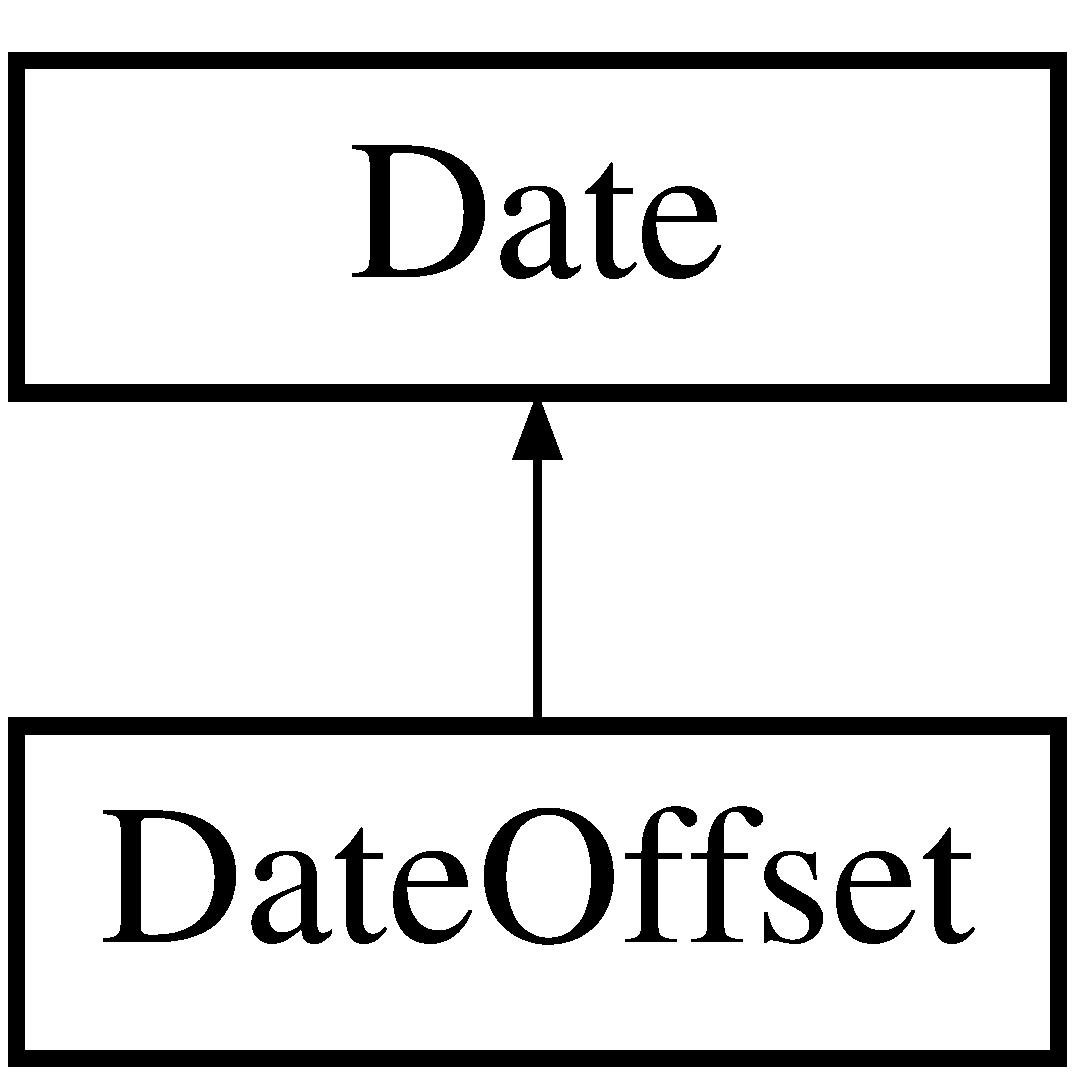
\includegraphics[height=2.000000cm]{class_date_offset}
\end{center}
\end{figure}
\subsection*{Public Member Functions}
\begin{DoxyCompactItemize}
\item 
\hyperlink{class_date_offset_ae7d276dad52a8e2e64a57f5071f935da}{Date\+Offset} ()
\begin{DoxyCompactList}\small\item\em This is the default \hyperlink{class_date_offset}{Date\+Offset} constructor. \end{DoxyCompactList}\item 
\hyperlink{class_date_offset_a5e213fb54c765571a947813a29fa5de2}{Date\+Offset} (const \hyperlink{class_date}{Date} \&)
\begin{DoxyCompactList}\small\item\em This is a copy constructor. \end{DoxyCompactList}\item 
\hyperlink{class_date_offset_aa4af09f70e978f2788462da2c640e491}{Date\+Offset} (const \hyperlink{class_date_offset}{Date\+Offset} \&)
\begin{DoxyCompactList}\small\item\em This is a copy constructor. \end{DoxyCompactList}\item 
\hyperlink{class_date_offset_a408a6346abbade92bd529a2173355854}{Date\+Offset} (int year, int month, int day)
\begin{DoxyCompactList}\small\item\em This is a non default constructor. \end{DoxyCompactList}\item 
\hyperlink{class_date_offset_a16163537e497743f3e8648be23150eef}{$\sim$\+Date\+Offset} ()
\begin{DoxyCompactList}\small\item\em This is the default \hyperlink{class_date_offset}{Date\+Offset} deconstructor. \end{DoxyCompactList}\item 
const \hyperlink{class_date_offset}{Date\+Offset} \hyperlink{class_date_offset_a64a1de182cdfb6b62cbde8893e0b211d}{operator-\/} () const 
\begin{DoxyCompactList}\small\item\em Overloaded Operator -\/. \end{DoxyCompactList}\end{DoxyCompactItemize}
\subsection*{Additional Inherited Members}


\subsection{Detailed Description}
C\+L\+A\+SS\+: \hyperlink{class_date_offset}{Date\+Offset} \+: public \hyperlink{class_date}{Date} 

 The \hyperlink{class_date_offset}{Date\+Offset} class will calculate for everytime there is a difference in the date class 

\subsection{Constructor \& Destructor Documentation}
\index{Date\+Offset@{Date\+Offset}!Date\+Offset@{Date\+Offset}}
\index{Date\+Offset@{Date\+Offset}!Date\+Offset@{Date\+Offset}}
\subsubsection[{\texorpdfstring{Date\+Offset()}{DateOffset()}}]{\setlength{\rightskip}{0pt plus 5cm}Date\+Offset\+::\+Date\+Offset (
\begin{DoxyParamCaption}
{}
\end{DoxyParamCaption}
)}\hypertarget{class_date_offset_ae7d276dad52a8e2e64a57f5071f935da}{}\label{class_date_offset_ae7d276dad52a8e2e64a57f5071f935da}


This is the default \hyperlink{class_date_offset}{Date\+Offset} constructor. 

This default constructor doesn\textquotesingle{}t effect the object \index{Date\+Offset@{Date\+Offset}!Date\+Offset@{Date\+Offset}}
\index{Date\+Offset@{Date\+Offset}!Date\+Offset@{Date\+Offset}}
\subsubsection[{\texorpdfstring{Date\+Offset(const Date \&)}{DateOffset(const Date &)}}]{\setlength{\rightskip}{0pt plus 5cm}Date\+Offset\+::\+Date\+Offset (
\begin{DoxyParamCaption}
\item[{const {\bf Date} \&}]{other}
\end{DoxyParamCaption}
)}\hypertarget{class_date_offset_a5e213fb54c765571a947813a29fa5de2}{}\label{class_date_offset_a5e213fb54c765571a947813a29fa5de2}


This is a copy constructor. 

This constructor will copy from another date object in to this new object \index{Date\+Offset@{Date\+Offset}!Date\+Offset@{Date\+Offset}}
\index{Date\+Offset@{Date\+Offset}!Date\+Offset@{Date\+Offset}}
\subsubsection[{\texorpdfstring{Date\+Offset(const Date\+Offset \&)}{DateOffset(const DateOffset &)}}]{\setlength{\rightskip}{0pt plus 5cm}Date\+Offset\+::\+Date\+Offset (
\begin{DoxyParamCaption}
\item[{const {\bf Date\+Offset} \&}]{other}
\end{DoxyParamCaption}
)}\hypertarget{class_date_offset_aa4af09f70e978f2788462da2c640e491}{}\label{class_date_offset_aa4af09f70e978f2788462da2c640e491}


This is a copy constructor. 

This constructor will copy from another \hyperlink{class_date_offset}{Date\+Offset} object in to this new object \index{Date\+Offset@{Date\+Offset}!Date\+Offset@{Date\+Offset}}
\index{Date\+Offset@{Date\+Offset}!Date\+Offset@{Date\+Offset}}
\subsubsection[{\texorpdfstring{Date\+Offset(int year, int month, int day)}{DateOffset(int year, int month, int day)}}]{\setlength{\rightskip}{0pt plus 5cm}Date\+Offset\+::\+Date\+Offset (
\begin{DoxyParamCaption}
\item[{int}]{year, }
\item[{int}]{month, }
\item[{int}]{day}
\end{DoxyParamCaption}
)}\hypertarget{class_date_offset_a408a6346abbade92bd529a2173355854}{}\label{class_date_offset_a408a6346abbade92bd529a2173355854}


This is a non default constructor. 

This constructor read in individual year, month, and day variables and store them in the private data members \index{Date\+Offset@{Date\+Offset}!````~Date\+Offset@{$\sim$\+Date\+Offset}}
\index{````~Date\+Offset@{$\sim$\+Date\+Offset}!Date\+Offset@{Date\+Offset}}
\subsubsection[{\texorpdfstring{$\sim$\+Date\+Offset()}{~DateOffset()}}]{\setlength{\rightskip}{0pt plus 5cm}Date\+Offset\+::$\sim$\+Date\+Offset (
\begin{DoxyParamCaption}
{}
\end{DoxyParamCaption}
)}\hypertarget{class_date_offset_a16163537e497743f3e8648be23150eef}{}\label{class_date_offset_a16163537e497743f3e8648be23150eef}


This is the default \hyperlink{class_date_offset}{Date\+Offset} deconstructor. 

This default deconstructor doesn\textquotesingle{}t effect the object 

\subsection{Member Function Documentation}
\index{Date\+Offset@{Date\+Offset}!operator-\/@{operator-\/}}
\index{operator-\/@{operator-\/}!Date\+Offset@{Date\+Offset}}
\subsubsection[{\texorpdfstring{operator-\/() const }{operator-() const }}]{\setlength{\rightskip}{0pt plus 5cm}const {\bf Date\+Offset} Date\+Offset\+::operator-\/ (
\begin{DoxyParamCaption}
{}
\end{DoxyParamCaption}
) const}\hypertarget{class_date_offset_a64a1de182cdfb6b62cbde8893e0b211d}{}\label{class_date_offset_a64a1de182cdfb6b62cbde8893e0b211d}


Overloaded Operator -\/. 

This operator returns the private data members of the date offset object in a \hyperlink{class_date_offset}{Date\+Offset} format 

The documentation for this class was generated from the following files\+:\begin{DoxyCompactItemize}
\item 
Date.\+h\item 
Date.\+cpp\end{DoxyCompactItemize}

\hypertarget{class_item}{}\section{Item Class Reference}
\label{class_item}\index{Item@{Item}}


{\ttfamily \#include $<$Item.\+h$>$}

\subsection*{Classes}
\begin{DoxyCompactItemize}
\item 
class \hyperlink{class_item_1_1_purchase}{Purchase}
\end{DoxyCompactItemize}
\subsection*{Public Member Functions}
\begin{DoxyCompactItemize}
\item 
\hyperlink{class_item_a297720c02984eab37332ae795d22189d}{Item} ()
\begin{DoxyCompactList}\small\item\em This is the default \hyperlink{class_item}{Item} constructor. \end{DoxyCompactList}\item 
\hyperlink{class_item_afc899efe46f7dc6d85e461cb2ca9ebaf}{Item} (const \hyperlink{class_item}{Item} \&)
\begin{DoxyCompactList}\small\item\em This is the \hyperlink{class_item}{Item} copy constructor. \end{DoxyCompactList}\item 
\hyperlink{class_item_a344bcf40797aec4d8504b5eeb116d03d}{Item} (int id, const Q\+String \&name, int quantity)
\begin{DoxyCompactList}\small\item\em This is a nondefault constructor. \end{DoxyCompactList}\item 
\hyperlink{class_item_ad0cc8be6fae78de7c88f937265fcf9de}{Item} (int id, const Q\+String \&name, int quantity, bool is\+On\+Shelf)
\begin{DoxyCompactList}\small\item\em This is a nondefault constructor. \end{DoxyCompactList}\item 
\hyperlink{class_item_a11663c84075b78c3ae5e30fdfcd7c458}{$\sim$\+Item} ()
\begin{DoxyCompactList}\small\item\em This is the default deconstructor. \end{DoxyCompactList}\item 
int \hyperlink{class_item_a44199628f22d918876d21c415a545b0d}{Id} () const 
\begin{DoxyCompactList}\small\item\em Id return. \end{DoxyCompactList}\item 
Q\+String \hyperlink{class_item_a591cfd33ce61df595047b45a4fdec052}{Name} () const 
\begin{DoxyCompactList}\small\item\em Name return. \end{DoxyCompactList}\item 
int \hyperlink{class_item_a2fe9750d2081ea58d178e1d4d7200eda}{Quantity} () const 
\begin{DoxyCompactList}\small\item\em Quantity return. \end{DoxyCompactList}\item 
bool \hyperlink{class_item_a782f7033019bf2dffe30d27dc830d446}{On\+Shelf} () const 
\begin{DoxyCompactList}\small\item\em On\+Shelf return. \end{DoxyCompactList}\item 
void \hyperlink{class_item_a0894d05d3d755dfae05494f1a8c6ed75}{Change\+Name} (const Q\+String \&)
\begin{DoxyCompactList}\small\item\em Changes the name variable. \end{DoxyCompactList}\item 
\hyperlink{class_item_1_1_purchase}{Purchase} \hyperlink{class_item_ab7b5bcc75c974fdf2f9b6f07098e8754}{Sell} (\hyperlink{class_member}{Member} \&customer, int quantity, const \hyperlink{class_date}{Date} \&date\+Of\+Sale)
\begin{DoxyCompactList}\small\item\em Returns a a purchase. \end{DoxyCompactList}\item 
\hyperlink{class_item_1_1_purchase}{Purchase} \hyperlink{class_item_a7465f0baad50838b38c23911f52ee9a6}{Sell} (\hyperlink{class_member}{Member} \&customer, int quantity, int year, int month, int day)
\begin{DoxyCompactList}\small\item\em Returns a a purchase. \end{DoxyCompactList}\item 
void \hyperlink{class_item_afc6aeeca0e43ca1c3513b0370fd40670}{Restock} (int)
\begin{DoxyCompactList}\small\item\em Restocks the item. \end{DoxyCompactList}\item 
void \hyperlink{class_item_ae2744222e97a9b4623be795abfcd7094}{On\+Shelf} (bool)
\begin{DoxyCompactList}\small\item\em Updates the On\+Shelf variable. \end{DoxyCompactList}\item 
void \hyperlink{class_item_a91f7b7b763838c9d806eef30d0e70bfc}{Deshelve} ()
\begin{DoxyCompactList}\small\item\em Sets the On\+Shelf variable. \end{DoxyCompactList}\item 
void \hyperlink{class_item_abb31702d0e49dbaa5f7f7e53ca081698}{Reshelve} ()
\begin{DoxyCompactList}\small\item\em Sets the On\+Shelf variable. \end{DoxyCompactList}\end{DoxyCompactItemize}


\subsection{Detailed Description}
C\+L\+A\+SS\+: \hyperlink{class_item}{Item} 

 The \hyperlink{class_item}{Item} class is able to keep track of one instance of an item, including the item\textquotesingle{}s id, name, quantity, and if it is on the shelf or not. 

\subsection{Constructor \& Destructor Documentation}
\index{Item@{Item}!Item@{Item}}
\index{Item@{Item}!Item@{Item}}
\subsubsection[{\texorpdfstring{Item()}{Item()}}]{\setlength{\rightskip}{0pt plus 5cm}Item\+::\+Item (
\begin{DoxyParamCaption}
{}
\end{DoxyParamCaption}
)}\hypertarget{class_item_a297720c02984eab37332ae795d22189d}{}\label{class_item_a297720c02984eab37332ae795d22189d}


This is the default \hyperlink{class_item}{Item} constructor. 

This constructor initializes the private variables for the object \index{Item@{Item}!Item@{Item}}
\index{Item@{Item}!Item@{Item}}
\subsubsection[{\texorpdfstring{Item(const Item \&)}{Item(const Item &)}}]{\setlength{\rightskip}{0pt plus 5cm}Item\+::\+Item (
\begin{DoxyParamCaption}
\item[{const {\bf Item} \&}]{other}
\end{DoxyParamCaption}
)}\hypertarget{class_item_afc899efe46f7dc6d85e461cb2ca9ebaf}{}\label{class_item_afc899efe46f7dc6d85e461cb2ca9ebaf}


This is the \hyperlink{class_item}{Item} copy constructor. 

This constructor copies the information from another object to this object \index{Item@{Item}!Item@{Item}}
\index{Item@{Item}!Item@{Item}}
\subsubsection[{\texorpdfstring{Item(int id, const Q\+String \&name, int quantity)}{Item(int id, const QString &name, int quantity)}}]{\setlength{\rightskip}{0pt plus 5cm}Item\+::\+Item (
\begin{DoxyParamCaption}
\item[{int}]{id, }
\item[{const Q\+String \&}]{name, }
\item[{int}]{quantity}
\end{DoxyParamCaption}
)}\hypertarget{class_item_a344bcf40797aec4d8504b5eeb116d03d}{}\label{class_item_a344bcf40797aec4d8504b5eeb116d03d}


This is a nondefault constructor. 

This constructor initializes the private data members from the arguemts as well as it initializes the is\+On\+Shelf variable to true \index{Item@{Item}!Item@{Item}}
\index{Item@{Item}!Item@{Item}}
\subsubsection[{\texorpdfstring{Item(int id, const Q\+String \&name, int quantity, bool is\+On\+Shelf)}{Item(int id, const QString &name, int quantity, bool isOnShelf)}}]{\setlength{\rightskip}{0pt plus 5cm}Item\+::\+Item (
\begin{DoxyParamCaption}
\item[{int}]{id, }
\item[{const Q\+String \&}]{name, }
\item[{int}]{quantity, }
\item[{bool}]{is\+On\+Shelf}
\end{DoxyParamCaption}
)}\hypertarget{class_item_ad0cc8be6fae78de7c88f937265fcf9de}{}\label{class_item_ad0cc8be6fae78de7c88f937265fcf9de}


This is a nondefault constructor. 

This constructor initializes the private data members from the arguemts \index{Item@{Item}!````~Item@{$\sim$\+Item}}
\index{````~Item@{$\sim$\+Item}!Item@{Item}}
\subsubsection[{\texorpdfstring{$\sim$\+Item()}{~Item()}}]{\setlength{\rightskip}{0pt plus 5cm}Item\+::$\sim$\+Item (
\begin{DoxyParamCaption}
{}
\end{DoxyParamCaption}
)}\hypertarget{class_item_a11663c84075b78c3ae5e30fdfcd7c458}{}\label{class_item_a11663c84075b78c3ae5e30fdfcd7c458}


This is the default deconstructor. 

This deconstructor doesn\textquotesingle{}t effect the object at all because there is no dynamic data being used in the object 

\subsection{Member Function Documentation}
\index{Item@{Item}!Change\+Name@{Change\+Name}}
\index{Change\+Name@{Change\+Name}!Item@{Item}}
\subsubsection[{\texorpdfstring{Change\+Name(const Q\+String \&)}{ChangeName(const QString &)}}]{\setlength{\rightskip}{0pt plus 5cm}void Item\+::\+Change\+Name (
\begin{DoxyParamCaption}
\item[{const Q\+String \&}]{name}
\end{DoxyParamCaption}
)}\hypertarget{class_item_a0894d05d3d755dfae05494f1a8c6ed75}{}\label{class_item_a0894d05d3d755dfae05494f1a8c6ed75}


Changes the name variable. 

This function uses the argument to update the name variable \index{Item@{Item}!Deshelve@{Deshelve}}
\index{Deshelve@{Deshelve}!Item@{Item}}
\subsubsection[{\texorpdfstring{Deshelve()}{Deshelve()}}]{\setlength{\rightskip}{0pt plus 5cm}void Item\+::\+Deshelve (
\begin{DoxyParamCaption}
{}
\end{DoxyParamCaption}
)}\hypertarget{class_item_a91f7b7b763838c9d806eef30d0e70bfc}{}\label{class_item_a91f7b7b763838c9d806eef30d0e70bfc}


Sets the On\+Shelf variable. 

Sets the On\+Shelf variable to false \index{Item@{Item}!Id@{Id}}
\index{Id@{Id}!Item@{Item}}
\subsubsection[{\texorpdfstring{Id() const }{Id() const }}]{\setlength{\rightskip}{0pt plus 5cm}int Item\+::\+Id (
\begin{DoxyParamCaption}
{}
\end{DoxyParamCaption}
) const}\hypertarget{class_item_a44199628f22d918876d21c415a545b0d}{}\label{class_item_a44199628f22d918876d21c415a545b0d}


Id return. 

Returns the Id \index{Item@{Item}!Name@{Name}}
\index{Name@{Name}!Item@{Item}}
\subsubsection[{\texorpdfstring{Name() const }{Name() const }}]{\setlength{\rightskip}{0pt plus 5cm}Q\+String Item\+::\+Name (
\begin{DoxyParamCaption}
{}
\end{DoxyParamCaption}
) const}\hypertarget{class_item_a591cfd33ce61df595047b45a4fdec052}{}\label{class_item_a591cfd33ce61df595047b45a4fdec052}


Name return. 

Returns the Name \index{Item@{Item}!On\+Shelf@{On\+Shelf}}
\index{On\+Shelf@{On\+Shelf}!Item@{Item}}
\subsubsection[{\texorpdfstring{On\+Shelf() const }{OnShelf() const }}]{\setlength{\rightskip}{0pt plus 5cm}bool Item\+::\+On\+Shelf (
\begin{DoxyParamCaption}
{}
\end{DoxyParamCaption}
) const}\hypertarget{class_item_a782f7033019bf2dffe30d27dc830d446}{}\label{class_item_a782f7033019bf2dffe30d27dc830d446}


On\+Shelf return. 

Returns the On\+Shelf \index{Item@{Item}!On\+Shelf@{On\+Shelf}}
\index{On\+Shelf@{On\+Shelf}!Item@{Item}}
\subsubsection[{\texorpdfstring{On\+Shelf(bool)}{OnShelf(bool)}}]{\setlength{\rightskip}{0pt plus 5cm}void Item\+::\+On\+Shelf (
\begin{DoxyParamCaption}
\item[{bool}]{is\+On\+Shelf}
\end{DoxyParamCaption}
)}\hypertarget{class_item_ae2744222e97a9b4623be795abfcd7094}{}\label{class_item_ae2744222e97a9b4623be795abfcd7094}


Updates the On\+Shelf variable. 

This function sets the On\+Shelf variable to the argument \index{Item@{Item}!Quantity@{Quantity}}
\index{Quantity@{Quantity}!Item@{Item}}
\subsubsection[{\texorpdfstring{Quantity() const }{Quantity() const }}]{\setlength{\rightskip}{0pt plus 5cm}int Item\+::\+Quantity (
\begin{DoxyParamCaption}
{}
\end{DoxyParamCaption}
) const}\hypertarget{class_item_a2fe9750d2081ea58d178e1d4d7200eda}{}\label{class_item_a2fe9750d2081ea58d178e1d4d7200eda}


Quantity return. 

Returns the Quantity \index{Item@{Item}!Reshelve@{Reshelve}}
\index{Reshelve@{Reshelve}!Item@{Item}}
\subsubsection[{\texorpdfstring{Reshelve()}{Reshelve()}}]{\setlength{\rightskip}{0pt plus 5cm}void Item\+::\+Reshelve (
\begin{DoxyParamCaption}
{}
\end{DoxyParamCaption}
)}\hypertarget{class_item_abb31702d0e49dbaa5f7f7e53ca081698}{}\label{class_item_abb31702d0e49dbaa5f7f7e53ca081698}


Sets the On\+Shelf variable. 

Sets the On\+Shelf variable to true \index{Item@{Item}!Restock@{Restock}}
\index{Restock@{Restock}!Item@{Item}}
\subsubsection[{\texorpdfstring{Restock(int)}{Restock(int)}}]{\setlength{\rightskip}{0pt plus 5cm}void Item\+::\+Restock (
\begin{DoxyParamCaption}
\item[{int}]{addend}
\end{DoxyParamCaption}
)}\hypertarget{class_item_afc6aeeca0e43ca1c3513b0370fd40670}{}\label{class_item_afc6aeeca0e43ca1c3513b0370fd40670}


Restocks the item. 

This function restocks the item and adds the argument to the quantity in stock \index{Item@{Item}!Sell@{Sell}}
\index{Sell@{Sell}!Item@{Item}}
\subsubsection[{\texorpdfstring{Sell(\+Member \&customer, int quantity, const Date \&date\+Of\+Sale)}{Sell(Member &customer, int quantity, const Date &dateOfSale)}}]{\setlength{\rightskip}{0pt plus 5cm}{\bf Item\+::\+Purchase} Item\+::\+Sell (
\begin{DoxyParamCaption}
\item[{{\bf Member} \&}]{customer, }
\item[{int}]{quantity, }
\item[{const {\bf Date} \&}]{date\+Of\+Sale}
\end{DoxyParamCaption}
)}\hypertarget{class_item_ab7b5bcc75c974fdf2f9b6f07098e8754}{}\label{class_item_ab7b5bcc75c974fdf2f9b6f07098e8754}


Returns a a purchase. 

This function uses the arguments to create a purchase that is returned from the function \index{Item@{Item}!Sell@{Sell}}
\index{Sell@{Sell}!Item@{Item}}
\subsubsection[{\texorpdfstring{Sell(\+Member \&customer, int quantity, int year, int month, int day)}{Sell(Member &customer, int quantity, int year, int month, int day)}}]{\setlength{\rightskip}{0pt plus 5cm}{\bf Item\+::\+Purchase} Item\+::\+Sell (
\begin{DoxyParamCaption}
\item[{{\bf Member} \&}]{customer, }
\item[{int}]{quantity, }
\item[{int}]{year, }
\item[{int}]{month, }
\item[{int}]{day}
\end{DoxyParamCaption}
)}\hypertarget{class_item_a7465f0baad50838b38c23911f52ee9a6}{}\label{class_item_a7465f0baad50838b38c23911f52ee9a6}


Returns a a purchase. 

This function uses the arguments to create a purchase that is returned from the function 

The documentation for this class was generated from the following files\+:\begin{DoxyCompactItemize}
\item 
Item.\+h\item 
Item.\+cpp\end{DoxyCompactItemize}

\hypertarget{class_member}{}\section{Member Class Reference}
\label{class_member}\index{Member@{Member}}


Keeps track of all of the aspects of a member.  




{\ttfamily \#include $<$Member.\+h$>$}

\subsection*{Public Member Functions}
\begin{DoxyCompactItemize}
\item 
\hyperlink{class_member_a44241aa6aa9b792b550d9cc29e7ad050}{Member} ()
\begin{DoxyCompactList}\small\item\em This is a default constructor. \end{DoxyCompactList}\item 
\hyperlink{class_member_aaba53c848d96f8612112bf13401ad1ef}{Member} (int id, const Q\+String \&name, float spent, const \hyperlink{class_date}{Date} \&expires)
\begin{DoxyCompactList}\small\item\em This is a nondefault constructor. \end{DoxyCompactList}\item 
\hyperlink{class_member_a83f3b1e6044c453f100090e5135327b2}{Member} (int id, const Q\+String \&name, float spent, int year, int month, int day)
\begin{DoxyCompactList}\small\item\em This is a nondefault constructor. \end{DoxyCompactList}\item 
\hyperlink{class_member_a045f335f95c4d4d46ddf59b715a822a0}{Member} (int id, const Q\+String \&name, float spent, bool premium, const \hyperlink{class_date}{Date} \&expires)
\begin{DoxyCompactList}\small\item\em This is a nondefault constructor. \end{DoxyCompactList}\item 
\hyperlink{class_member_a8635ea86acc412cb9dedf7773f01b0fb}{Member} (int id, const Q\+String \&name, float spent, bool premium, int year, int month, int day)
\begin{DoxyCompactList}\small\item\em This is a nondefault constructor. \end{DoxyCompactList}\item 
virtual \hyperlink{class_member_a9e993260f63c73a91f1cb9b55fcef903}{$\sim$\+Member} ()
\begin{DoxyCompactList}\small\item\em This is a virtual deconstructor. \end{DoxyCompactList}\item 
int \hyperlink{class_member_ade792a4814b246281de4fe2a5017e5d6}{Id} () const 
\begin{DoxyCompactList}\small\item\em Id return. \end{DoxyCompactList}\item 
Q\+String \hyperlink{class_member_a5bac99875876ae00c127d47aa69370ff}{Name} () const 
\begin{DoxyCompactList}\small\item\em Name return. \end{DoxyCompactList}\item 
\hyperlink{class_date}{Date} \hyperlink{class_member_a38d327ef94499ef08c51b8a4791d6974}{Expires} () const 
\begin{DoxyCompactList}\small\item\em Expires return. \end{DoxyCompactList}\item 
bool \hyperlink{class_member_acc79ba154fd76148d5c34c3df7f0f1bf}{Premium} () const 
\begin{DoxyCompactList}\small\item\em Premium return. \end{DoxyCompactList}\item 
double \hyperlink{class_member_aa34e695e052dbdaf47f39388d524b9ee}{Spent} () const 
\begin{DoxyCompactList}\small\item\em Spent return. \end{DoxyCompactList}\item 
double \hyperlink{class_member_ab6a428e16603847fb696a9a5c90f9143}{Rebate} () const 
\begin{DoxyCompactList}\small\item\em Rebate return. \end{DoxyCompactList}\item 
bool \hyperlink{class_member_ab51d2e131d03ed0120648cce975b77d1}{Active} () const 
\begin{DoxyCompactList}\small\item\em Active return. \end{DoxyCompactList}\item 
void \hyperlink{class_member_a1003f8aaaf3d11141a642fe3a330527d}{Change\+Name} (const Q\+String \&)
\begin{DoxyCompactList}\small\item\em Changes the name of the member. \end{DoxyCompactList}\item 
void \hyperlink{class_member_a00269243882b9e39dacfdcbcc885c307}{Set\+Active} (bool is\+Active)
\begin{DoxyCompactList}\small\item\em Changes the active membership of the member. \end{DoxyCompactList}\item 
void \hyperlink{class_member_a835b9172cfe0a9ab0ad23c8843175562}{Upgrade\+Membership} ()
\begin{DoxyCompactList}\small\item\em Upgrades the member\textquotesingle{}s membership. \end{DoxyCompactList}\item 
void \hyperlink{class_member_a87fe6a012352d66c332c8a4f36c58c0c}{Downgrade\+Membership} ()
\begin{DoxyCompactList}\small\item\em Downgrades the member\textquotesingle{}s membership. \end{DoxyCompactList}\item 
void \hyperlink{class_member_a13fe2db5fd5eee4754c4d55ee0dd7ef5}{Change\+Expiration\+Date} (const \hyperlink{class_date}{Date} \&)
\begin{DoxyCompactList}\small\item\em Changes the expiration date of the membership. \end{DoxyCompactList}\item 
void \hyperlink{class_member_a520c6c140590c66aa2d9b60aada1b684}{Change\+Expiration\+Date} (int year, int month, int day)
\begin{DoxyCompactList}\small\item\em Changes the expiration date of the membership. \end{DoxyCompactList}\end{DoxyCompactItemize}


\subsection{Detailed Description}
Keeps track of all of the aspects of a member. 

C\+L\+A\+SS\+: \hyperlink{class_member}{Member} 

 The \hyperlink{class_member}{Member} class keeps track of a member, including the id, name, spent, premium, expires, and the active membership of the member 

\subsection{Constructor \& Destructor Documentation}
\index{Member@{Member}!Member@{Member}}
\index{Member@{Member}!Member@{Member}}
\subsubsection[{\texorpdfstring{Member()}{Member()}}]{\setlength{\rightskip}{0pt plus 5cm}Member\+::\+Member (
\begin{DoxyParamCaption}
{}
\end{DoxyParamCaption}
)}\hypertarget{class_member_a44241aa6aa9b792b550d9cc29e7ad050}{}\label{class_member_a44241aa6aa9b792b550d9cc29e7ad050}


This is a default constructor. 

This constructor will initialize the variables \index{Member@{Member}!Member@{Member}}
\index{Member@{Member}!Member@{Member}}
\subsubsection[{\texorpdfstring{Member(int id, const Q\+String \&name, float spent, const Date \&expires)}{Member(int id, const QString &name, float spent, const Date &expires)}}]{\setlength{\rightskip}{0pt plus 5cm}Member\+::\+Member (
\begin{DoxyParamCaption}
\item[{int}]{id, }
\item[{const Q\+String \&}]{name, }
\item[{float}]{spent, }
\item[{const {\bf Date} \&}]{expires}
\end{DoxyParamCaption}
)}\hypertarget{class_member_aaba53c848d96f8612112bf13401ad1ef}{}\label{class_member_aaba53c848d96f8612112bf13401ad1ef}


This is a nondefault constructor. 

This constructor will initialize the variables from the arguments \index{Member@{Member}!Member@{Member}}
\index{Member@{Member}!Member@{Member}}
\subsubsection[{\texorpdfstring{Member(int id, const Q\+String \&name, float spent, int year, int month, int day)}{Member(int id, const QString &name, float spent, int year, int month, int day)}}]{\setlength{\rightskip}{0pt plus 5cm}Member\+::\+Member (
\begin{DoxyParamCaption}
\item[{int}]{id, }
\item[{const Q\+String \&}]{name, }
\item[{float}]{spent, }
\item[{int}]{year, }
\item[{int}]{month, }
\item[{int}]{day}
\end{DoxyParamCaption}
)}\hypertarget{class_member_a83f3b1e6044c453f100090e5135327b2}{}\label{class_member_a83f3b1e6044c453f100090e5135327b2}


This is a nondefault constructor. 

This constructor will initialize the variables from the arguments \index{Member@{Member}!Member@{Member}}
\index{Member@{Member}!Member@{Member}}
\subsubsection[{\texorpdfstring{Member(int id, const Q\+String \&name, float spent, bool premium, const Date \&expires)}{Member(int id, const QString &name, float spent, bool premium, const Date &expires)}}]{\setlength{\rightskip}{0pt plus 5cm}Member\+::\+Member (
\begin{DoxyParamCaption}
\item[{int}]{id, }
\item[{const Q\+String \&}]{name, }
\item[{float}]{spent, }
\item[{bool}]{premium, }
\item[{const {\bf Date} \&}]{expires}
\end{DoxyParamCaption}
)}\hypertarget{class_member_a045f335f95c4d4d46ddf59b715a822a0}{}\label{class_member_a045f335f95c4d4d46ddf59b715a822a0}


This is a nondefault constructor. 

This constructor will initialize the variables from the arguments \index{Member@{Member}!Member@{Member}}
\index{Member@{Member}!Member@{Member}}
\subsubsection[{\texorpdfstring{Member(int id, const Q\+String \&name, float spent, bool premium, int year, int month, int day)}{Member(int id, const QString &name, float spent, bool premium, int year, int month, int day)}}]{\setlength{\rightskip}{0pt plus 5cm}Member\+::\+Member (
\begin{DoxyParamCaption}
\item[{int}]{id, }
\item[{const Q\+String \&}]{name, }
\item[{float}]{spent, }
\item[{bool}]{premium, }
\item[{int}]{year, }
\item[{int}]{month, }
\item[{int}]{day}
\end{DoxyParamCaption}
)}\hypertarget{class_member_a8635ea86acc412cb9dedf7773f01b0fb}{}\label{class_member_a8635ea86acc412cb9dedf7773f01b0fb}


This is a nondefault constructor. 

This constructor will initialize the variables from the arguments \index{Member@{Member}!````~Member@{$\sim$\+Member}}
\index{````~Member@{$\sim$\+Member}!Member@{Member}}
\subsubsection[{\texorpdfstring{$\sim$\+Member()}{~Member()}}]{\setlength{\rightskip}{0pt plus 5cm}virtual Member\+::$\sim$\+Member (
\begin{DoxyParamCaption}
{}
\end{DoxyParamCaption}
)\hspace{0.3cm}{\ttfamily [virtual]}}\hypertarget{class_member_a9e993260f63c73a91f1cb9b55fcef903}{}\label{class_member_a9e993260f63c73a91f1cb9b55fcef903}


This is a virtual deconstructor. 

This deconstructor does nothing 

\subsection{Member Function Documentation}
\index{Member@{Member}!Active@{Active}}
\index{Active@{Active}!Member@{Member}}
\subsubsection[{\texorpdfstring{Active() const }{Active() const }}]{\setlength{\rightskip}{0pt plus 5cm}bool Member\+::\+Active (
\begin{DoxyParamCaption}
{}
\end{DoxyParamCaption}
) const}\hypertarget{class_member_ab51d2e131d03ed0120648cce975b77d1}{}\label{class_member_ab51d2e131d03ed0120648cce975b77d1}


Active return. 

This returns what the Active is pointing to \index{Member@{Member}!Change\+Expiration\+Date@{Change\+Expiration\+Date}}
\index{Change\+Expiration\+Date@{Change\+Expiration\+Date}!Member@{Member}}
\subsubsection[{\texorpdfstring{Change\+Expiration\+Date(const Date \&)}{ChangeExpirationDate(const Date &)}}]{\setlength{\rightskip}{0pt plus 5cm}void Member\+::\+Change\+Expiration\+Date (
\begin{DoxyParamCaption}
\item[{const {\bf Date} \&}]{}
\end{DoxyParamCaption}
)}\hypertarget{class_member_a13fe2db5fd5eee4754c4d55ee0dd7ef5}{}\label{class_member_a13fe2db5fd5eee4754c4d55ee0dd7ef5}


Changes the expiration date of the membership. 

This function uses the date argument to update the expiration date \index{Member@{Member}!Change\+Expiration\+Date@{Change\+Expiration\+Date}}
\index{Change\+Expiration\+Date@{Change\+Expiration\+Date}!Member@{Member}}
\subsubsection[{\texorpdfstring{Change\+Expiration\+Date(int year, int month, int day)}{ChangeExpirationDate(int year, int month, int day)}}]{\setlength{\rightskip}{0pt plus 5cm}void Member\+::\+Change\+Expiration\+Date (
\begin{DoxyParamCaption}
\item[{int}]{year, }
\item[{int}]{month, }
\item[{int}]{day}
\end{DoxyParamCaption}
)}\hypertarget{class_member_a520c6c140590c66aa2d9b60aada1b684}{}\label{class_member_a520c6c140590c66aa2d9b60aada1b684}


Changes the expiration date of the membership. 

This function uses the year, month, and day arguments to update the expiration date \index{Member@{Member}!Change\+Name@{Change\+Name}}
\index{Change\+Name@{Change\+Name}!Member@{Member}}
\subsubsection[{\texorpdfstring{Change\+Name(const Q\+String \&)}{ChangeName(const QString &)}}]{\setlength{\rightskip}{0pt plus 5cm}void Member\+::\+Change\+Name (
\begin{DoxyParamCaption}
\item[{const Q\+String \&}]{}
\end{DoxyParamCaption}
)}\hypertarget{class_member_a1003f8aaaf3d11141a642fe3a330527d}{}\label{class_member_a1003f8aaaf3d11141a642fe3a330527d}


Changes the name of the member. 

This function updates the member name \index{Member@{Member}!Downgrade\+Membership@{Downgrade\+Membership}}
\index{Downgrade\+Membership@{Downgrade\+Membership}!Member@{Member}}
\subsubsection[{\texorpdfstring{Downgrade\+Membership()}{DowngradeMembership()}}]{\setlength{\rightskip}{0pt plus 5cm}void Member\+::\+Downgrade\+Membership (
\begin{DoxyParamCaption}
{}
\end{DoxyParamCaption}
)}\hypertarget{class_member_a87fe6a012352d66c332c8a4f36c58c0c}{}\label{class_member_a87fe6a012352d66c332c8a4f36c58c0c}


Downgrades the member\textquotesingle{}s membership. 

This function sets the flag to false \index{Member@{Member}!Expires@{Expires}}
\index{Expires@{Expires}!Member@{Member}}
\subsubsection[{\texorpdfstring{Expires() const }{Expires() const }}]{\setlength{\rightskip}{0pt plus 5cm}{\bf Date} Member\+::\+Expires (
\begin{DoxyParamCaption}
{}
\end{DoxyParamCaption}
) const}\hypertarget{class_member_a38d327ef94499ef08c51b8a4791d6974}{}\label{class_member_a38d327ef94499ef08c51b8a4791d6974}


Expires return. 

This returns what the Expires is pointing to \index{Member@{Member}!Id@{Id}}
\index{Id@{Id}!Member@{Member}}
\subsubsection[{\texorpdfstring{Id() const }{Id() const }}]{\setlength{\rightskip}{0pt plus 5cm}int Member\+::\+Id (
\begin{DoxyParamCaption}
{}
\end{DoxyParamCaption}
) const}\hypertarget{class_member_ade792a4814b246281de4fe2a5017e5d6}{}\label{class_member_ade792a4814b246281de4fe2a5017e5d6}


Id return. 

This returns what the Id is pointing to \index{Member@{Member}!Name@{Name}}
\index{Name@{Name}!Member@{Member}}
\subsubsection[{\texorpdfstring{Name() const }{Name() const }}]{\setlength{\rightskip}{0pt plus 5cm}Q\+String Member\+::\+Name (
\begin{DoxyParamCaption}
{}
\end{DoxyParamCaption}
) const}\hypertarget{class_member_a5bac99875876ae00c127d47aa69370ff}{}\label{class_member_a5bac99875876ae00c127d47aa69370ff}


Name return. 

This returns what the Name is pointing to \index{Member@{Member}!Premium@{Premium}}
\index{Premium@{Premium}!Member@{Member}}
\subsubsection[{\texorpdfstring{Premium() const }{Premium() const }}]{\setlength{\rightskip}{0pt plus 5cm}bool Member\+::\+Premium (
\begin{DoxyParamCaption}
{}
\end{DoxyParamCaption}
) const}\hypertarget{class_member_acc79ba154fd76148d5c34c3df7f0f1bf}{}\label{class_member_acc79ba154fd76148d5c34c3df7f0f1bf}


Premium return. 

This returns what the Premium is pointing to \index{Member@{Member}!Rebate@{Rebate}}
\index{Rebate@{Rebate}!Member@{Member}}
\subsubsection[{\texorpdfstring{Rebate() const }{Rebate() const }}]{\setlength{\rightskip}{0pt plus 5cm}double Member\+::\+Rebate (
\begin{DoxyParamCaption}
{}
\end{DoxyParamCaption}
) const}\hypertarget{class_member_ab6a428e16603847fb696a9a5c90f9143}{}\label{class_member_ab6a428e16603847fb696a9a5c90f9143}


Rebate return. 

This returns what the Rebate is pointing to \index{Member@{Member}!Set\+Active@{Set\+Active}}
\index{Set\+Active@{Set\+Active}!Member@{Member}}
\subsubsection[{\texorpdfstring{Set\+Active(bool is\+Active)}{SetActive(bool isActive)}}]{\setlength{\rightskip}{0pt plus 5cm}void Member\+::\+Set\+Active (
\begin{DoxyParamCaption}
\item[{bool}]{is\+Active}
\end{DoxyParamCaption}
)}\hypertarget{class_member_a00269243882b9e39dacfdcbcc885c307}{}\label{class_member_a00269243882b9e39dacfdcbcc885c307}


Changes the active membership of the member. 

This function updates the member\textquotesingle{}s active membership \index{Member@{Member}!Spent@{Spent}}
\index{Spent@{Spent}!Member@{Member}}
\subsubsection[{\texorpdfstring{Spent() const }{Spent() const }}]{\setlength{\rightskip}{0pt plus 5cm}double Member\+::\+Spent (
\begin{DoxyParamCaption}
{}
\end{DoxyParamCaption}
) const}\hypertarget{class_member_aa34e695e052dbdaf47f39388d524b9ee}{}\label{class_member_aa34e695e052dbdaf47f39388d524b9ee}


Spent return. 

This returns what the Spent is pointing to \index{Member@{Member}!Upgrade\+Membership@{Upgrade\+Membership}}
\index{Upgrade\+Membership@{Upgrade\+Membership}!Member@{Member}}
\subsubsection[{\texorpdfstring{Upgrade\+Membership()}{UpgradeMembership()}}]{\setlength{\rightskip}{0pt plus 5cm}void Member\+::\+Upgrade\+Membership (
\begin{DoxyParamCaption}
{}
\end{DoxyParamCaption}
)}\hypertarget{class_member_a835b9172cfe0a9ab0ad23c8843175562}{}\label{class_member_a835b9172cfe0a9ab0ad23c8843175562}


Upgrades the member\textquotesingle{}s membership. 

This function sets the flag to true 

The documentation for this class was generated from the following file\+:\begin{DoxyCompactItemize}
\item 
Member.\+h\end{DoxyCompactItemize}

\hypertarget{class_purchase}{}\section{Purchase Class Reference}
\label{class_purchase}\index{Purchase@{Purchase}}


Maintains all of the information for a purchase.  




{\ttfamily \#include $<$Purchase.\+h$>$}

\subsection*{Public Member Functions}
\begin{DoxyCompactItemize}
\item 
\hyperlink{class_purchase_ad08eb8e99875d8973ecbeea1da3e175e}{Purchase} (int \hyperlink{class_purchase_ac11c5f5772648b8e5a8e1dd370982720}{ID}, \hyperlink{class_item}{Item} $\ast$\&item\+Ref, \hyperlink{class_member}{Member} $\ast$\&member\+Ref, int quantity, const \hyperlink{class_date}{Date} \&sale)
\begin{DoxyCompactList}\small\item\em This is a nondefault constructor. \end{DoxyCompactList}\item 
\hyperlink{class_purchase_a075ce333db37c0005559a4dac7afb32a}{Purchase} (int \hyperlink{class_purchase_ac11c5f5772648b8e5a8e1dd370982720}{ID}, \hyperlink{class_item}{Item} $\ast$\&item\+Ref, \hyperlink{class_member}{Member} $\ast$\&member\+Ref, int quantity, int year, int month, int day)
\begin{DoxyCompactList}\small\item\em This is a nondefault constructor. \end{DoxyCompactList}\item 
\hyperlink{class_purchase_a8ebd6efb2177df6d10fcba514095915f}{$\sim$\+Purchase} ()
\begin{DoxyCompactList}\small\item\em This is the default deconstructor. \end{DoxyCompactList}\item 
void {\bfseries Set\+ID} ()\hypertarget{class_purchase_ac23880f64fed84e2237e748bfda10acd}{}\label{class_purchase_ac23880f64fed84e2237e748bfda10acd}

\item 
\hyperlink{class_item}{Item} $\ast$\& \hyperlink{class_purchase_ae42cfec377bf8338185d21481654f126}{Item\+Ref} ()
\begin{DoxyCompactList}\small\item\em Item\+Ref return. \end{DoxyCompactList}\item 
\hyperlink{class_member}{Member} $\ast$\& \hyperlink{class_purchase_ac1b9c14867cc21b71cfd8a8a025d64e1}{Member\+Ref} ()
\begin{DoxyCompactList}\small\item\em Member\+Ref return. \end{DoxyCompactList}\item 
int \hyperlink{class_purchase_ac11c5f5772648b8e5a8e1dd370982720}{ID} () const 
\begin{DoxyCompactList}\small\item\em ID return. \end{DoxyCompactList}\item 
int \hyperlink{class_purchase_af8915f2329cb353968562a2ccaf9e0df}{Quantity} () const 
\begin{DoxyCompactList}\small\item\em Quantity return. \end{DoxyCompactList}\item 
\hyperlink{class_date}{Date} \hyperlink{class_purchase_ac69d08647056818ff0fc61dec674461f}{Date\+Of\+Sale} () const 
\begin{DoxyCompactList}\small\item\em Date\+Of\+Sale return. \end{DoxyCompactList}\end{DoxyCompactItemize}


\subsection{Detailed Description}
Maintains all of the information for a purchase. 

C\+L\+A\+SS\+: \hyperlink{class_purchase}{Purchase} 

 The \hyperlink{class_purchase}{Purchase} class keeps track of a current purchase, including the id, quantity, and sale date of the purchase. 

\subsection{Constructor \& Destructor Documentation}
\index{Purchase@{Purchase}!Purchase@{Purchase}}
\index{Purchase@{Purchase}!Purchase@{Purchase}}
\subsubsection[{\texorpdfstring{Purchase(int I\+D, Item $\ast$\&item\+Ref, Member $\ast$\&member\+Ref, int quantity, const Date \&sale)}{Purchase(int ID, Item *&itemRef, Member *&memberRef, int quantity, const Date &sale)}}]{\setlength{\rightskip}{0pt plus 5cm}Purchase\+::\+Purchase (
\begin{DoxyParamCaption}
\item[{int}]{ID, }
\item[{{\bf Item} $\ast$\&}]{item\+Ref, }
\item[{{\bf Member} $\ast$\&}]{member\+Ref, }
\item[{int}]{quantity, }
\item[{const {\bf Date} \&}]{sale}
\end{DoxyParamCaption}
)}\hypertarget{class_purchase_ad08eb8e99875d8973ecbeea1da3e175e}{}\label{class_purchase_ad08eb8e99875d8973ecbeea1da3e175e}


This is a nondefault constructor. 

This constructor will initialize the variables from the arguments \index{Purchase@{Purchase}!Purchase@{Purchase}}
\index{Purchase@{Purchase}!Purchase@{Purchase}}
\subsubsection[{\texorpdfstring{Purchase(int I\+D, Item $\ast$\&item\+Ref, Member $\ast$\&member\+Ref, int quantity, int year, int month, int day)}{Purchase(int ID, Item *&itemRef, Member *&memberRef, int quantity, int year, int month, int day)}}]{\setlength{\rightskip}{0pt plus 5cm}Purchase\+::\+Purchase (
\begin{DoxyParamCaption}
\item[{int}]{ID, }
\item[{{\bf Item} $\ast$\&}]{item\+Ref, }
\item[{{\bf Member} $\ast$\&}]{member\+Ref, }
\item[{int}]{quantity, }
\item[{int}]{year, }
\item[{int}]{month, }
\item[{int}]{day}
\end{DoxyParamCaption}
)}\hypertarget{class_purchase_a075ce333db37c0005559a4dac7afb32a}{}\label{class_purchase_a075ce333db37c0005559a4dac7afb32a}


This is a nondefault constructor. 

This constructor will initialize the variables from the arguments, except instead of copying the date object over, it reads in individual year, month, and day \index{Purchase@{Purchase}!````~Purchase@{$\sim$\+Purchase}}
\index{````~Purchase@{$\sim$\+Purchase}!Purchase@{Purchase}}
\subsubsection[{\texorpdfstring{$\sim$\+Purchase()}{~Purchase()}}]{\setlength{\rightskip}{0pt plus 5cm}Purchase\+::$\sim$\+Purchase (
\begin{DoxyParamCaption}
{}
\end{DoxyParamCaption}
)}\hypertarget{class_purchase_a8ebd6efb2177df6d10fcba514095915f}{}\label{class_purchase_a8ebd6efb2177df6d10fcba514095915f}


This is the default deconstructor. 

This deconstructor doesn\textquotesingle{}t effect the object at all because there is no dynamic data being used in the object 

\subsection{Member Function Documentation}
\index{Purchase@{Purchase}!Date\+Of\+Sale@{Date\+Of\+Sale}}
\index{Date\+Of\+Sale@{Date\+Of\+Sale}!Purchase@{Purchase}}
\subsubsection[{\texorpdfstring{Date\+Of\+Sale() const }{DateOfSale() const }}]{\setlength{\rightskip}{0pt plus 5cm}{\bf Date} Purchase\+::\+Date\+Of\+Sale (
\begin{DoxyParamCaption}
{}
\end{DoxyParamCaption}
) const}\hypertarget{class_purchase_ac69d08647056818ff0fc61dec674461f}{}\label{class_purchase_ac69d08647056818ff0fc61dec674461f}


Date\+Of\+Sale return. 

Returns the Date\+Of\+Sale \index{Purchase@{Purchase}!ID@{ID}}
\index{ID@{ID}!Purchase@{Purchase}}
\subsubsection[{\texorpdfstring{I\+D() const }{ID() const }}]{\setlength{\rightskip}{0pt plus 5cm}int Purchase\+::\+ID (
\begin{DoxyParamCaption}
{}
\end{DoxyParamCaption}
) const}\hypertarget{class_purchase_ac11c5f5772648b8e5a8e1dd370982720}{}\label{class_purchase_ac11c5f5772648b8e5a8e1dd370982720}


ID return. 

Returns the ID variable \index{Purchase@{Purchase}!Item\+Ref@{Item\+Ref}}
\index{Item\+Ref@{Item\+Ref}!Purchase@{Purchase}}
\subsubsection[{\texorpdfstring{Item\+Ref()}{ItemRef()}}]{\setlength{\rightskip}{0pt plus 5cm}{\bf Item}$\ast$\& Purchase\+::\+Item\+Ref (
\begin{DoxyParamCaption}
{}
\end{DoxyParamCaption}
)}\hypertarget{class_purchase_ae42cfec377bf8338185d21481654f126}{}\label{class_purchase_ae42cfec377bf8338185d21481654f126}


Item\+Ref return. 

This returns what the Item\+Ref is pointing to \index{Purchase@{Purchase}!Member\+Ref@{Member\+Ref}}
\index{Member\+Ref@{Member\+Ref}!Purchase@{Purchase}}
\subsubsection[{\texorpdfstring{Member\+Ref()}{MemberRef()}}]{\setlength{\rightskip}{0pt plus 5cm}{\bf Member}$\ast$\& Purchase\+::\+Member\+Ref (
\begin{DoxyParamCaption}
{}
\end{DoxyParamCaption}
)}\hypertarget{class_purchase_ac1b9c14867cc21b71cfd8a8a025d64e1}{}\label{class_purchase_ac1b9c14867cc21b71cfd8a8a025d64e1}


Member\+Ref return. 

This returns what the Member\+Ref is pointing to \index{Purchase@{Purchase}!Quantity@{Quantity}}
\index{Quantity@{Quantity}!Purchase@{Purchase}}
\subsubsection[{\texorpdfstring{Quantity() const }{Quantity() const }}]{\setlength{\rightskip}{0pt plus 5cm}int Purchase\+::\+Quantity (
\begin{DoxyParamCaption}
{}
\end{DoxyParamCaption}
) const}\hypertarget{class_purchase_af8915f2329cb353968562a2ccaf9e0df}{}\label{class_purchase_af8915f2329cb353968562a2ccaf9e0df}


Quantity return. 

Returns the Quantity 

The documentation for this class was generated from the following file\+:\begin{DoxyCompactItemize}
\item 
Purchase.\+h\end{DoxyCompactItemize}

%--- End generated contents ---

% Index
\backmatter
\newpage
\phantomsection
\clearemptydoublepage
\addcontentsline{toc}{chapter}{Index}
\printindex

\end{document}
